\begin{figure}
			\centering
			\subfloat[SHREK]{
				\scalebox{.4}{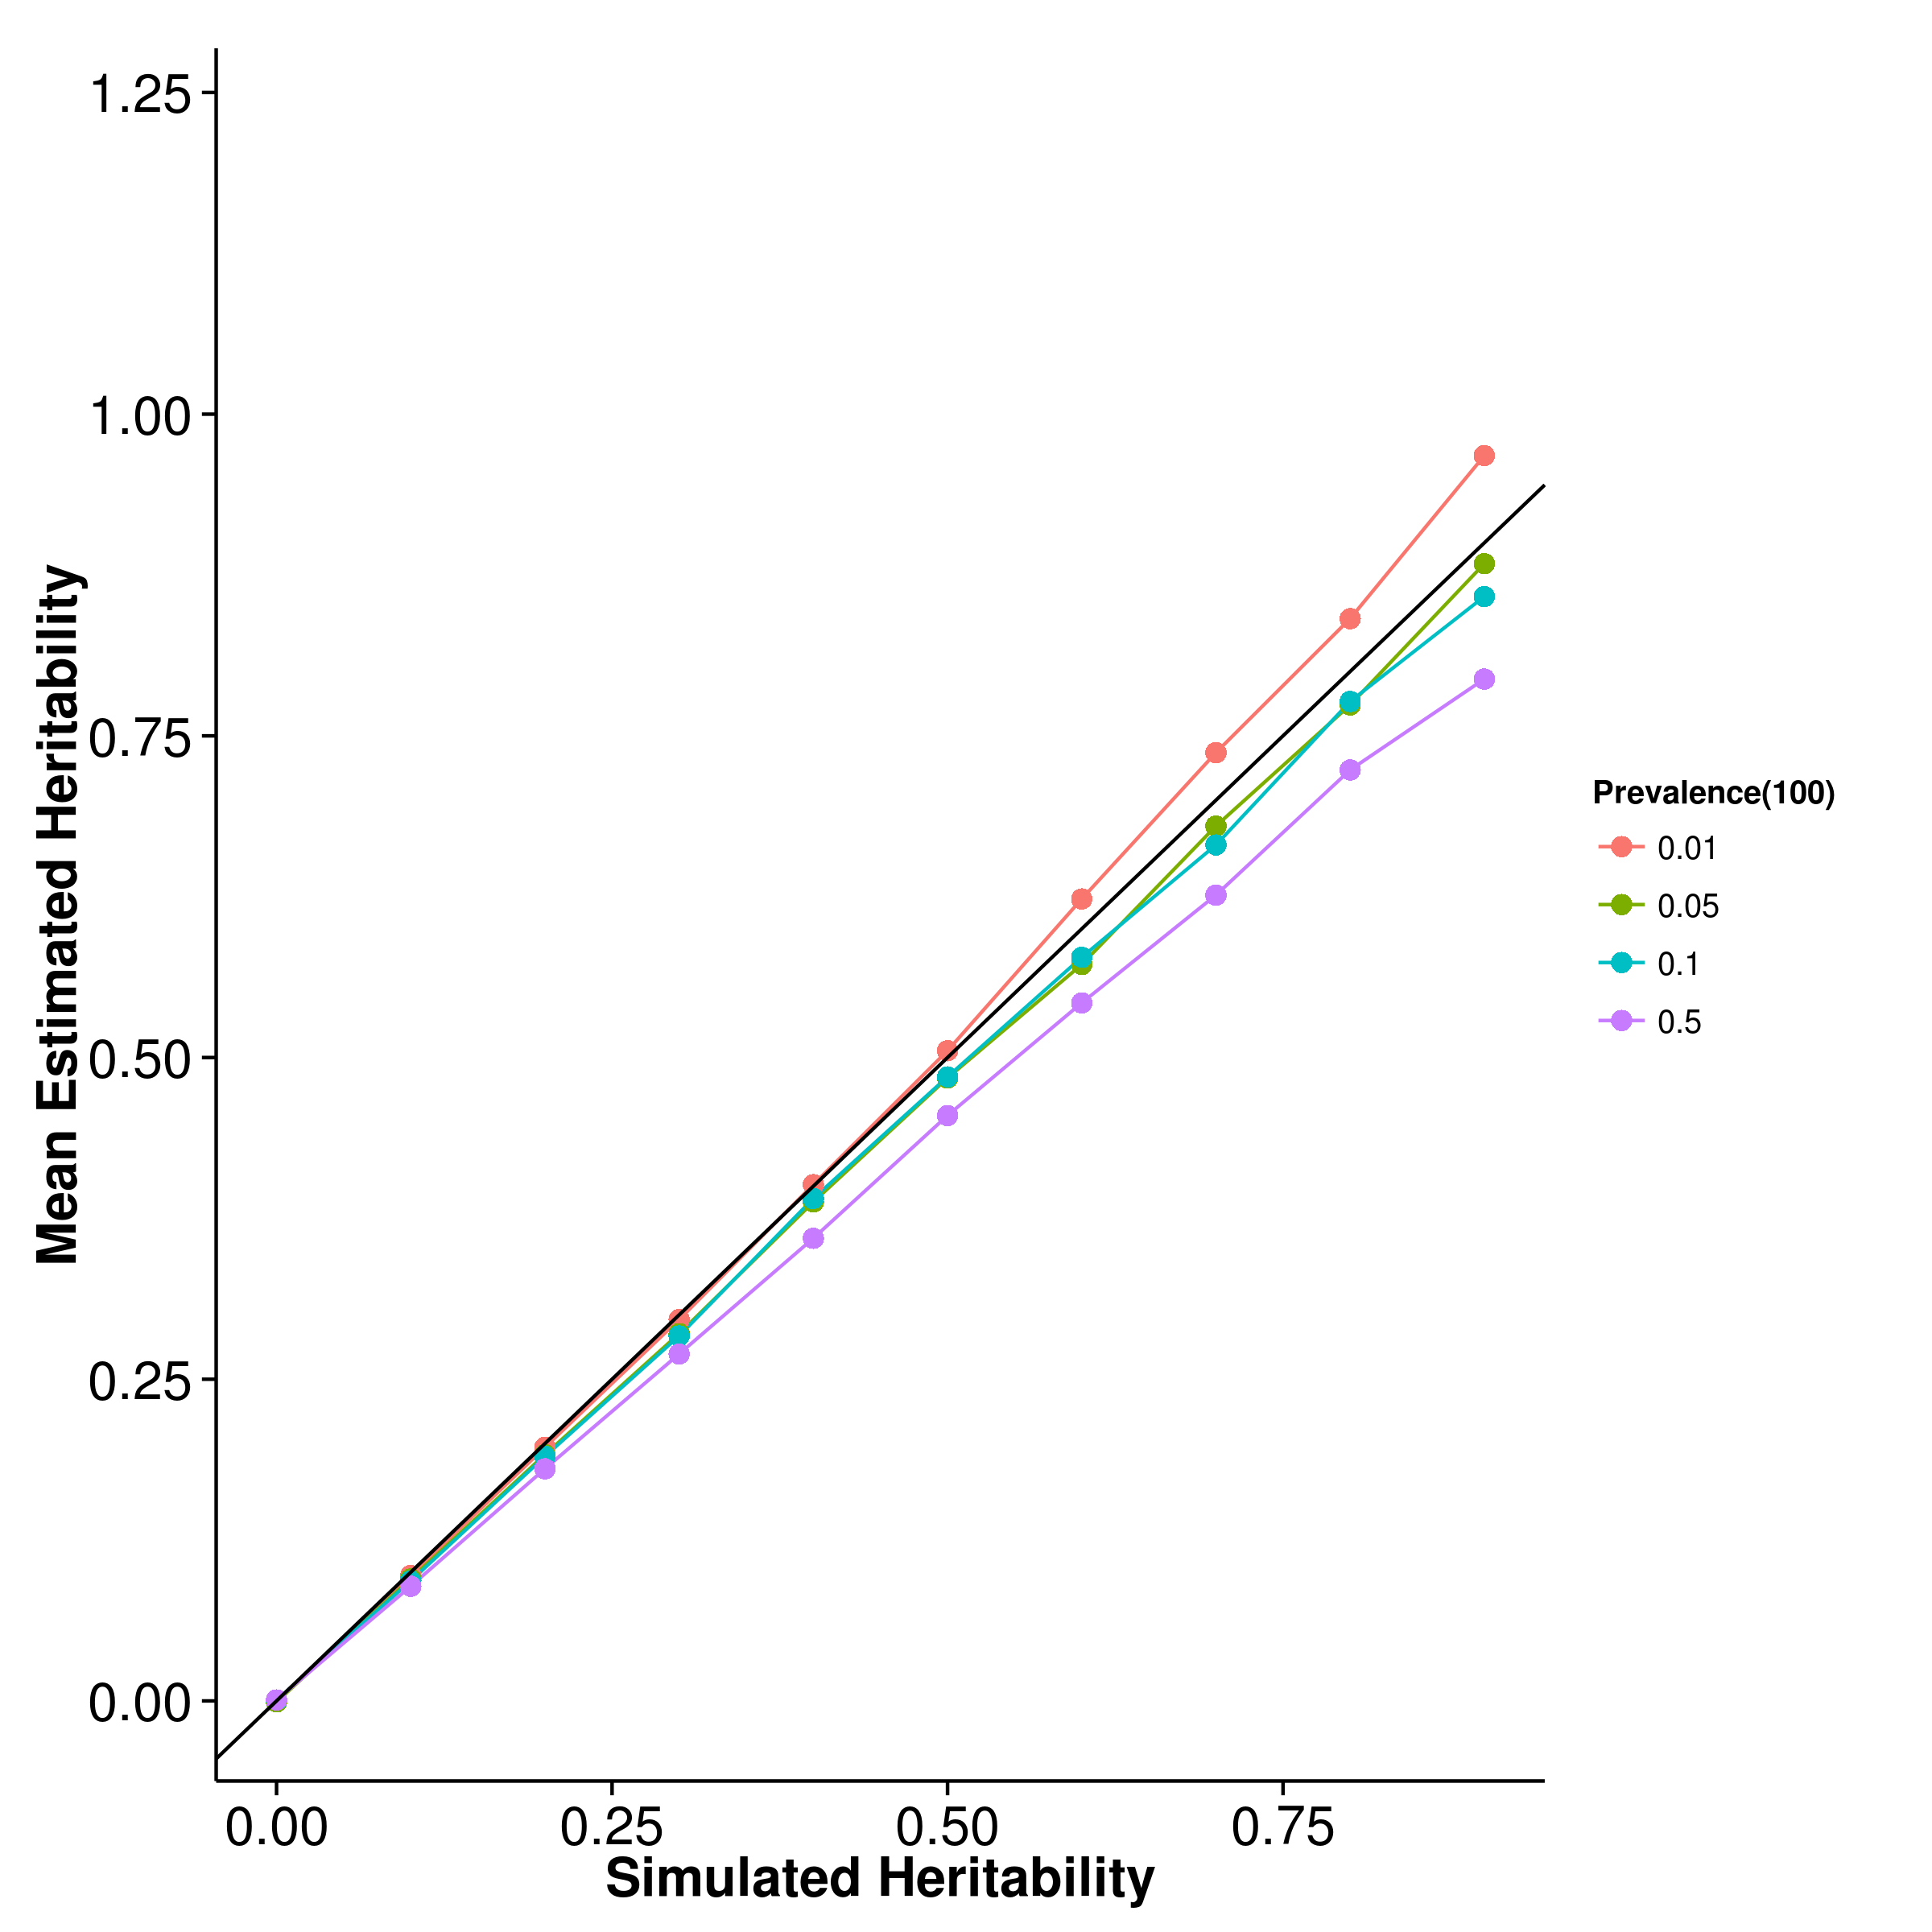
\includegraphics{figure/he_summary/cc_100c/shrek_CC_Random_mean.png}}
				\label{fig:shrekCCRandMean}
			}
			\subfloat[GCTA]{
				\scalebox{.4}{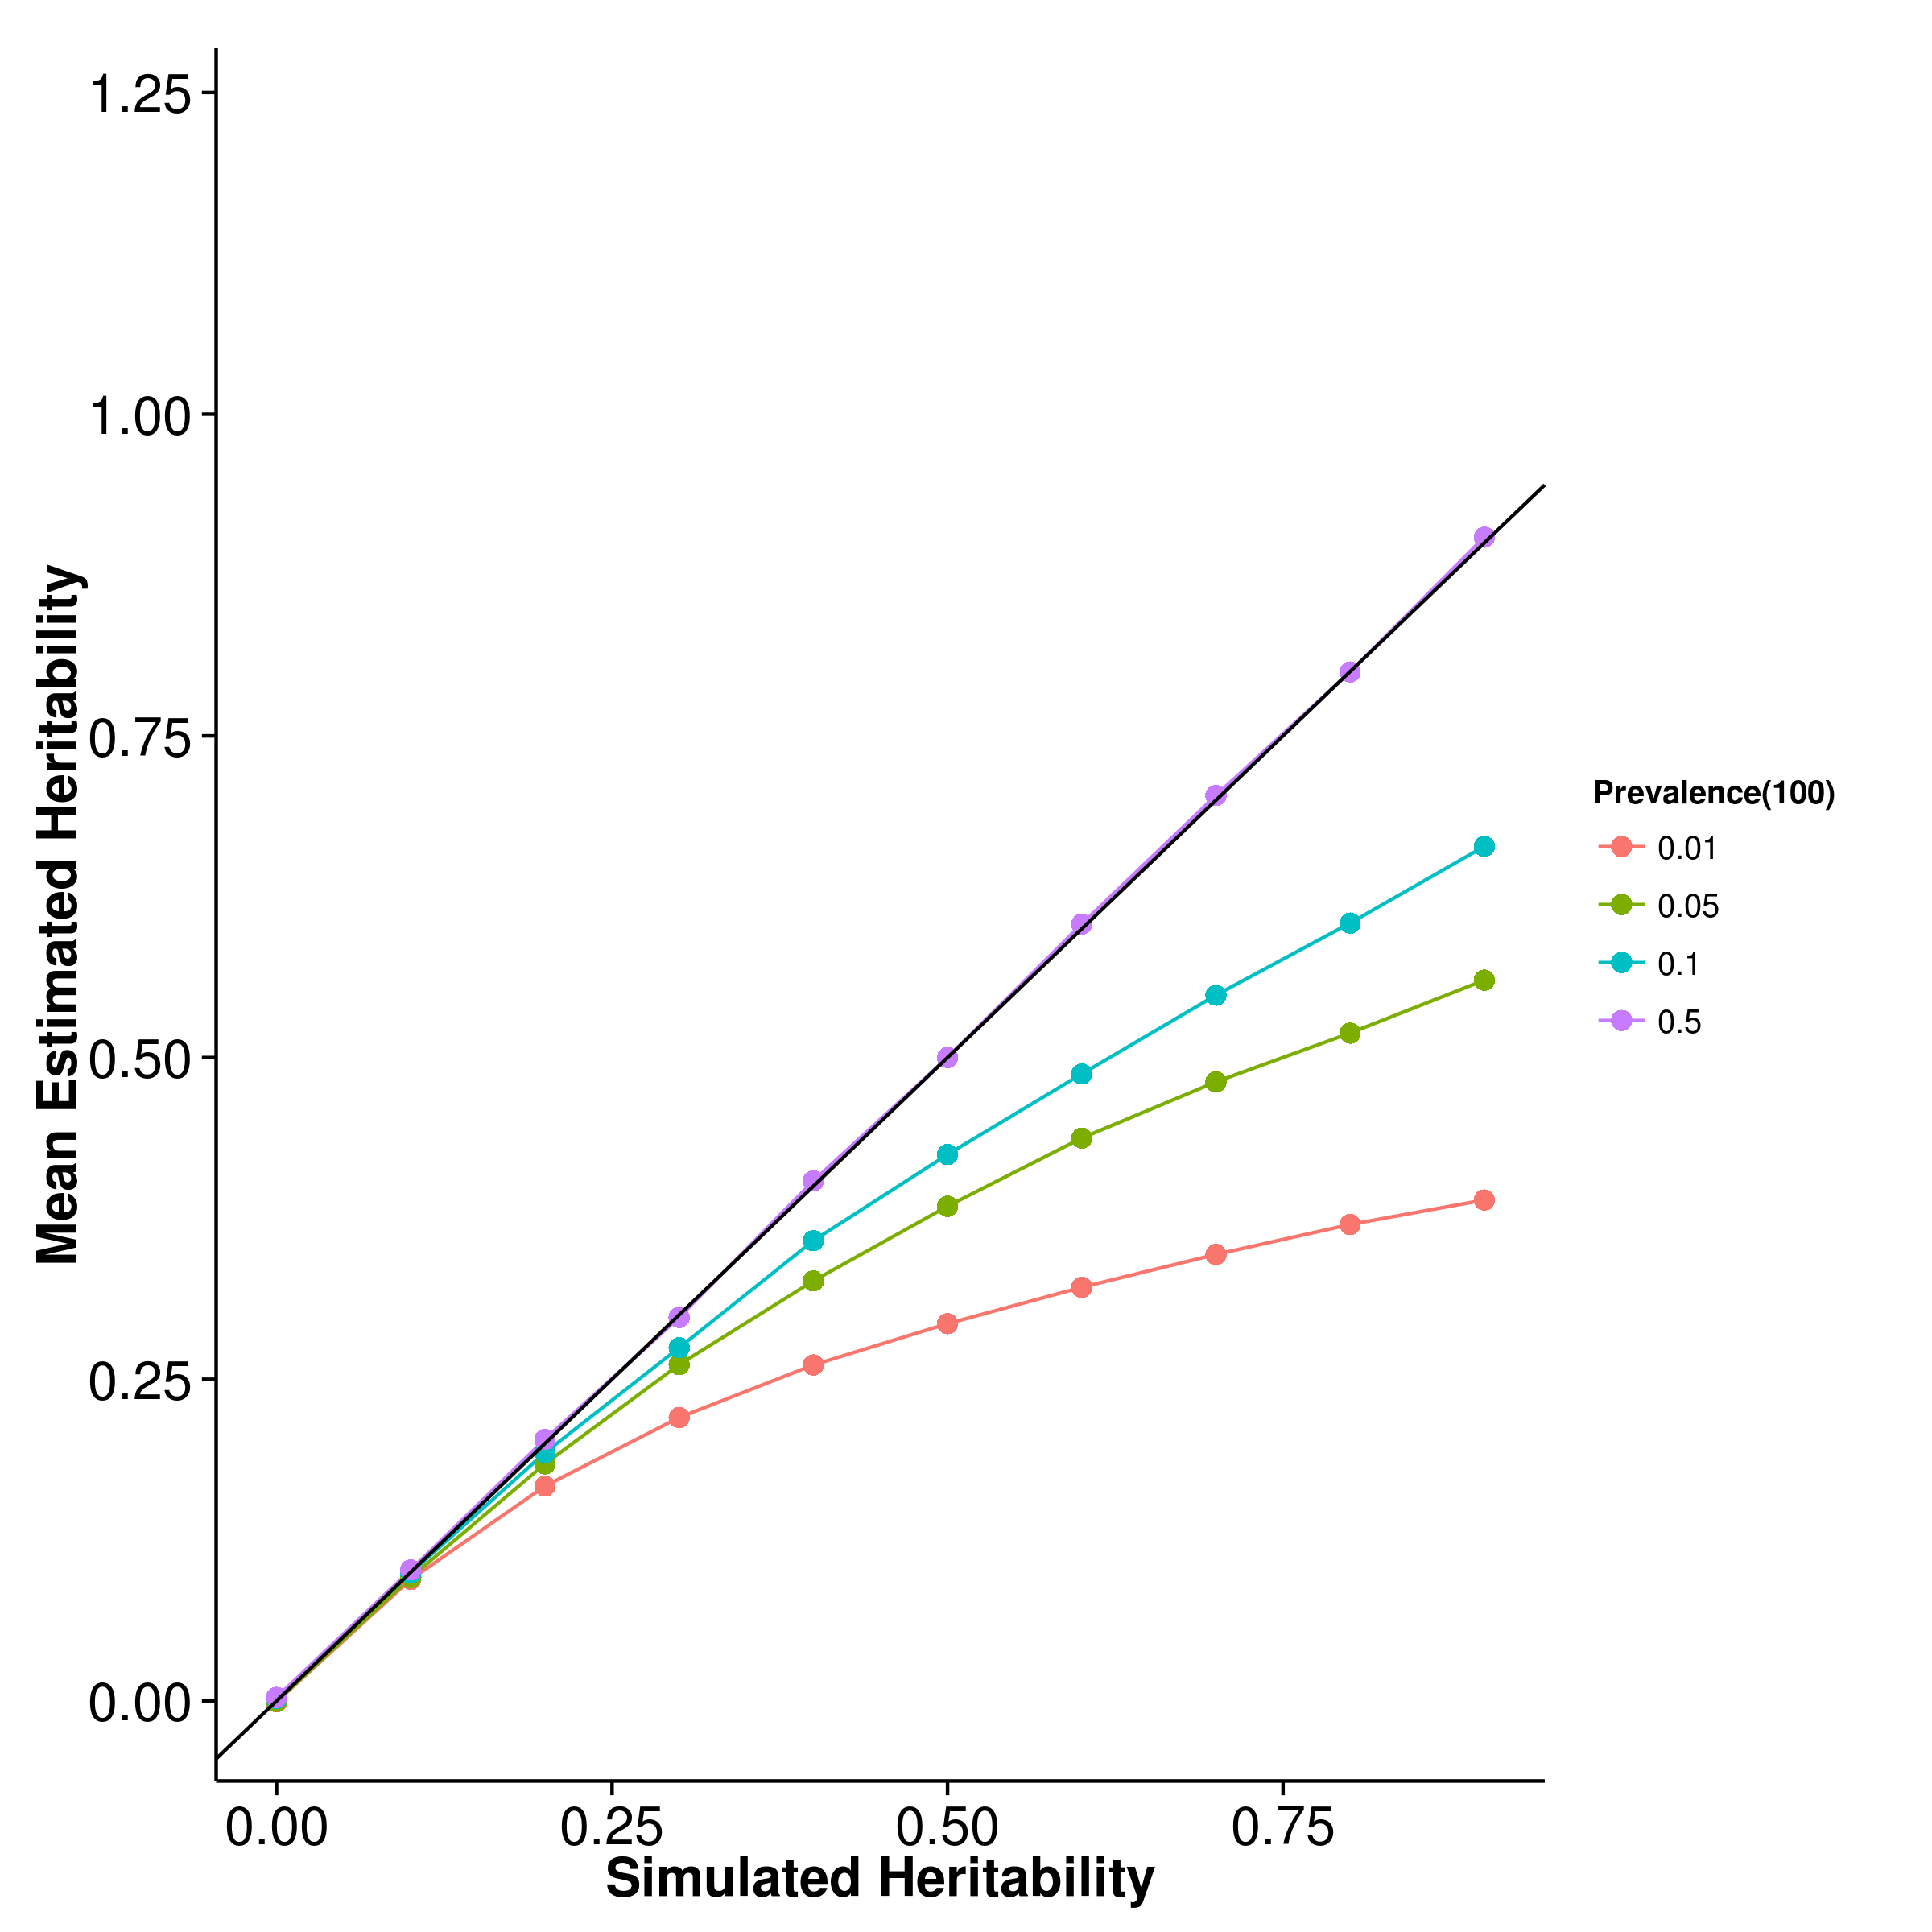
\includegraphics{figure/he_summary/cc_100c/gcta_CC_Random_mean.png}}
				\label{fig:gctaCCRandMean}
			}\\
			\subfloat[LDSC with fix intercept]{
				\scalebox{.4}{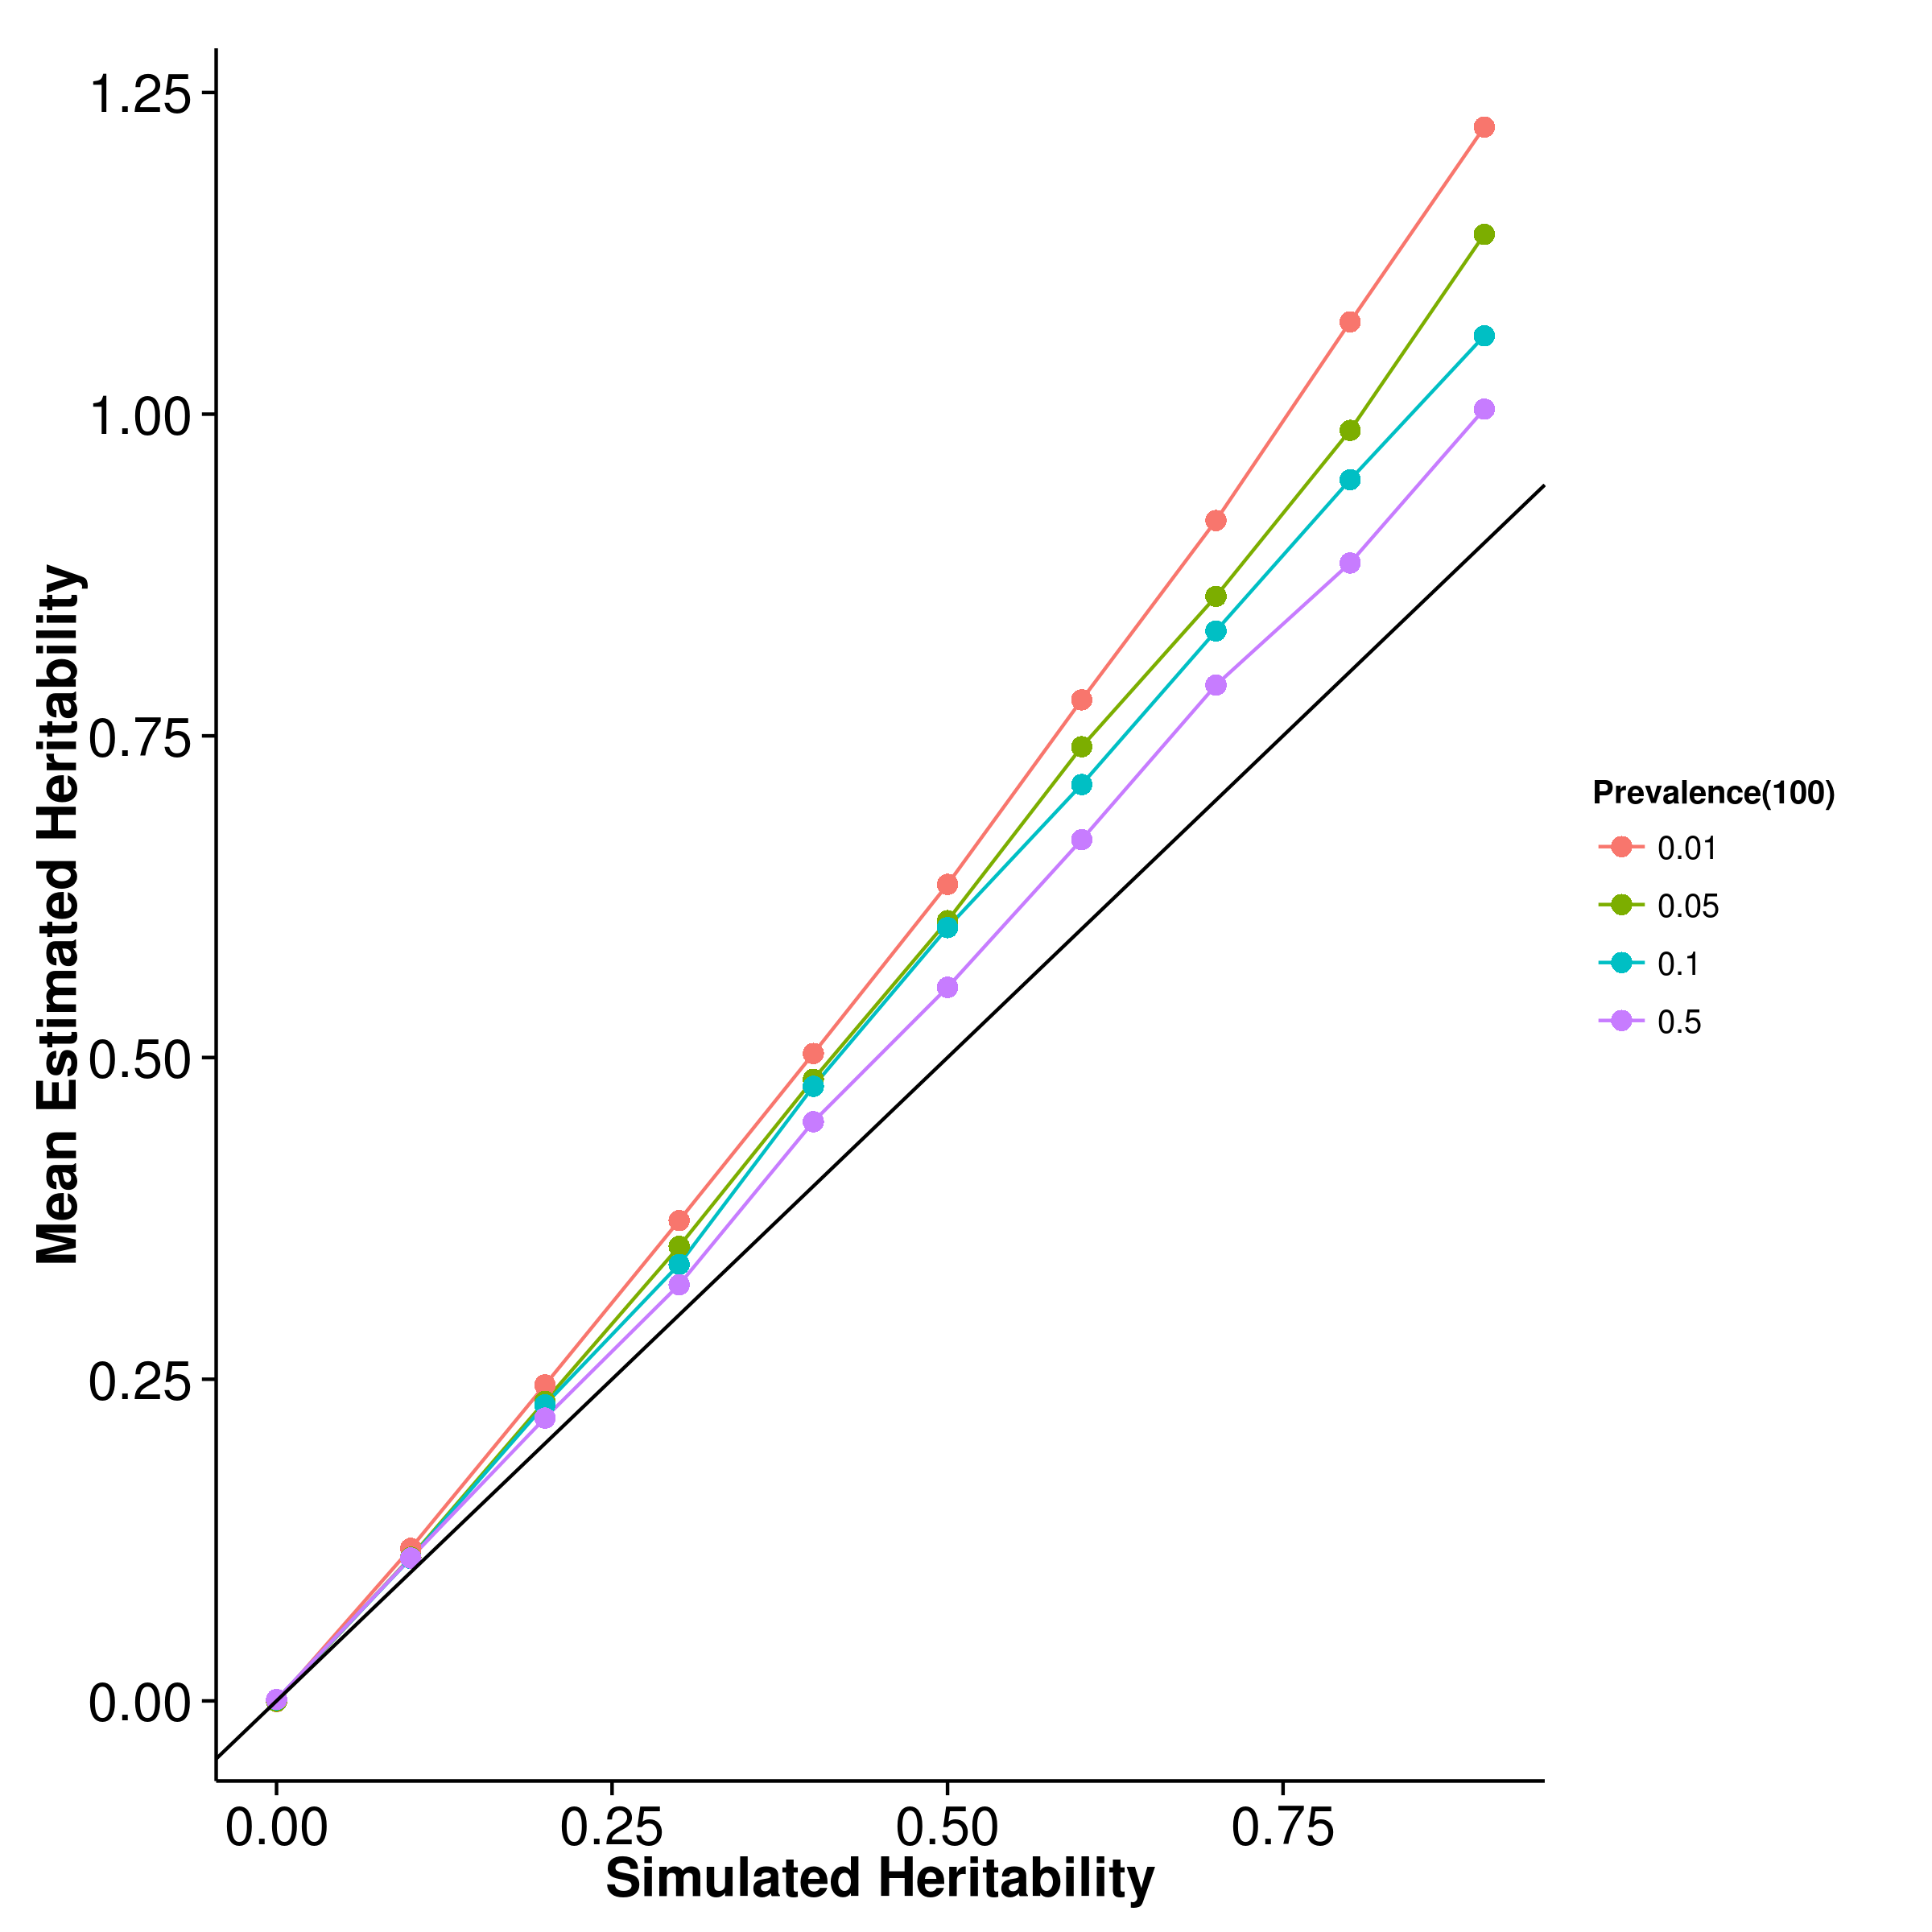
\includegraphics{figure/he_summary/cc_100c/ldsc_CC_Random_mean.png}}
				\label{fig:ldscCCRandMean}
			}
			\subfloat[LDSC with intercept estimation]{
				
				\scalebox{.4}{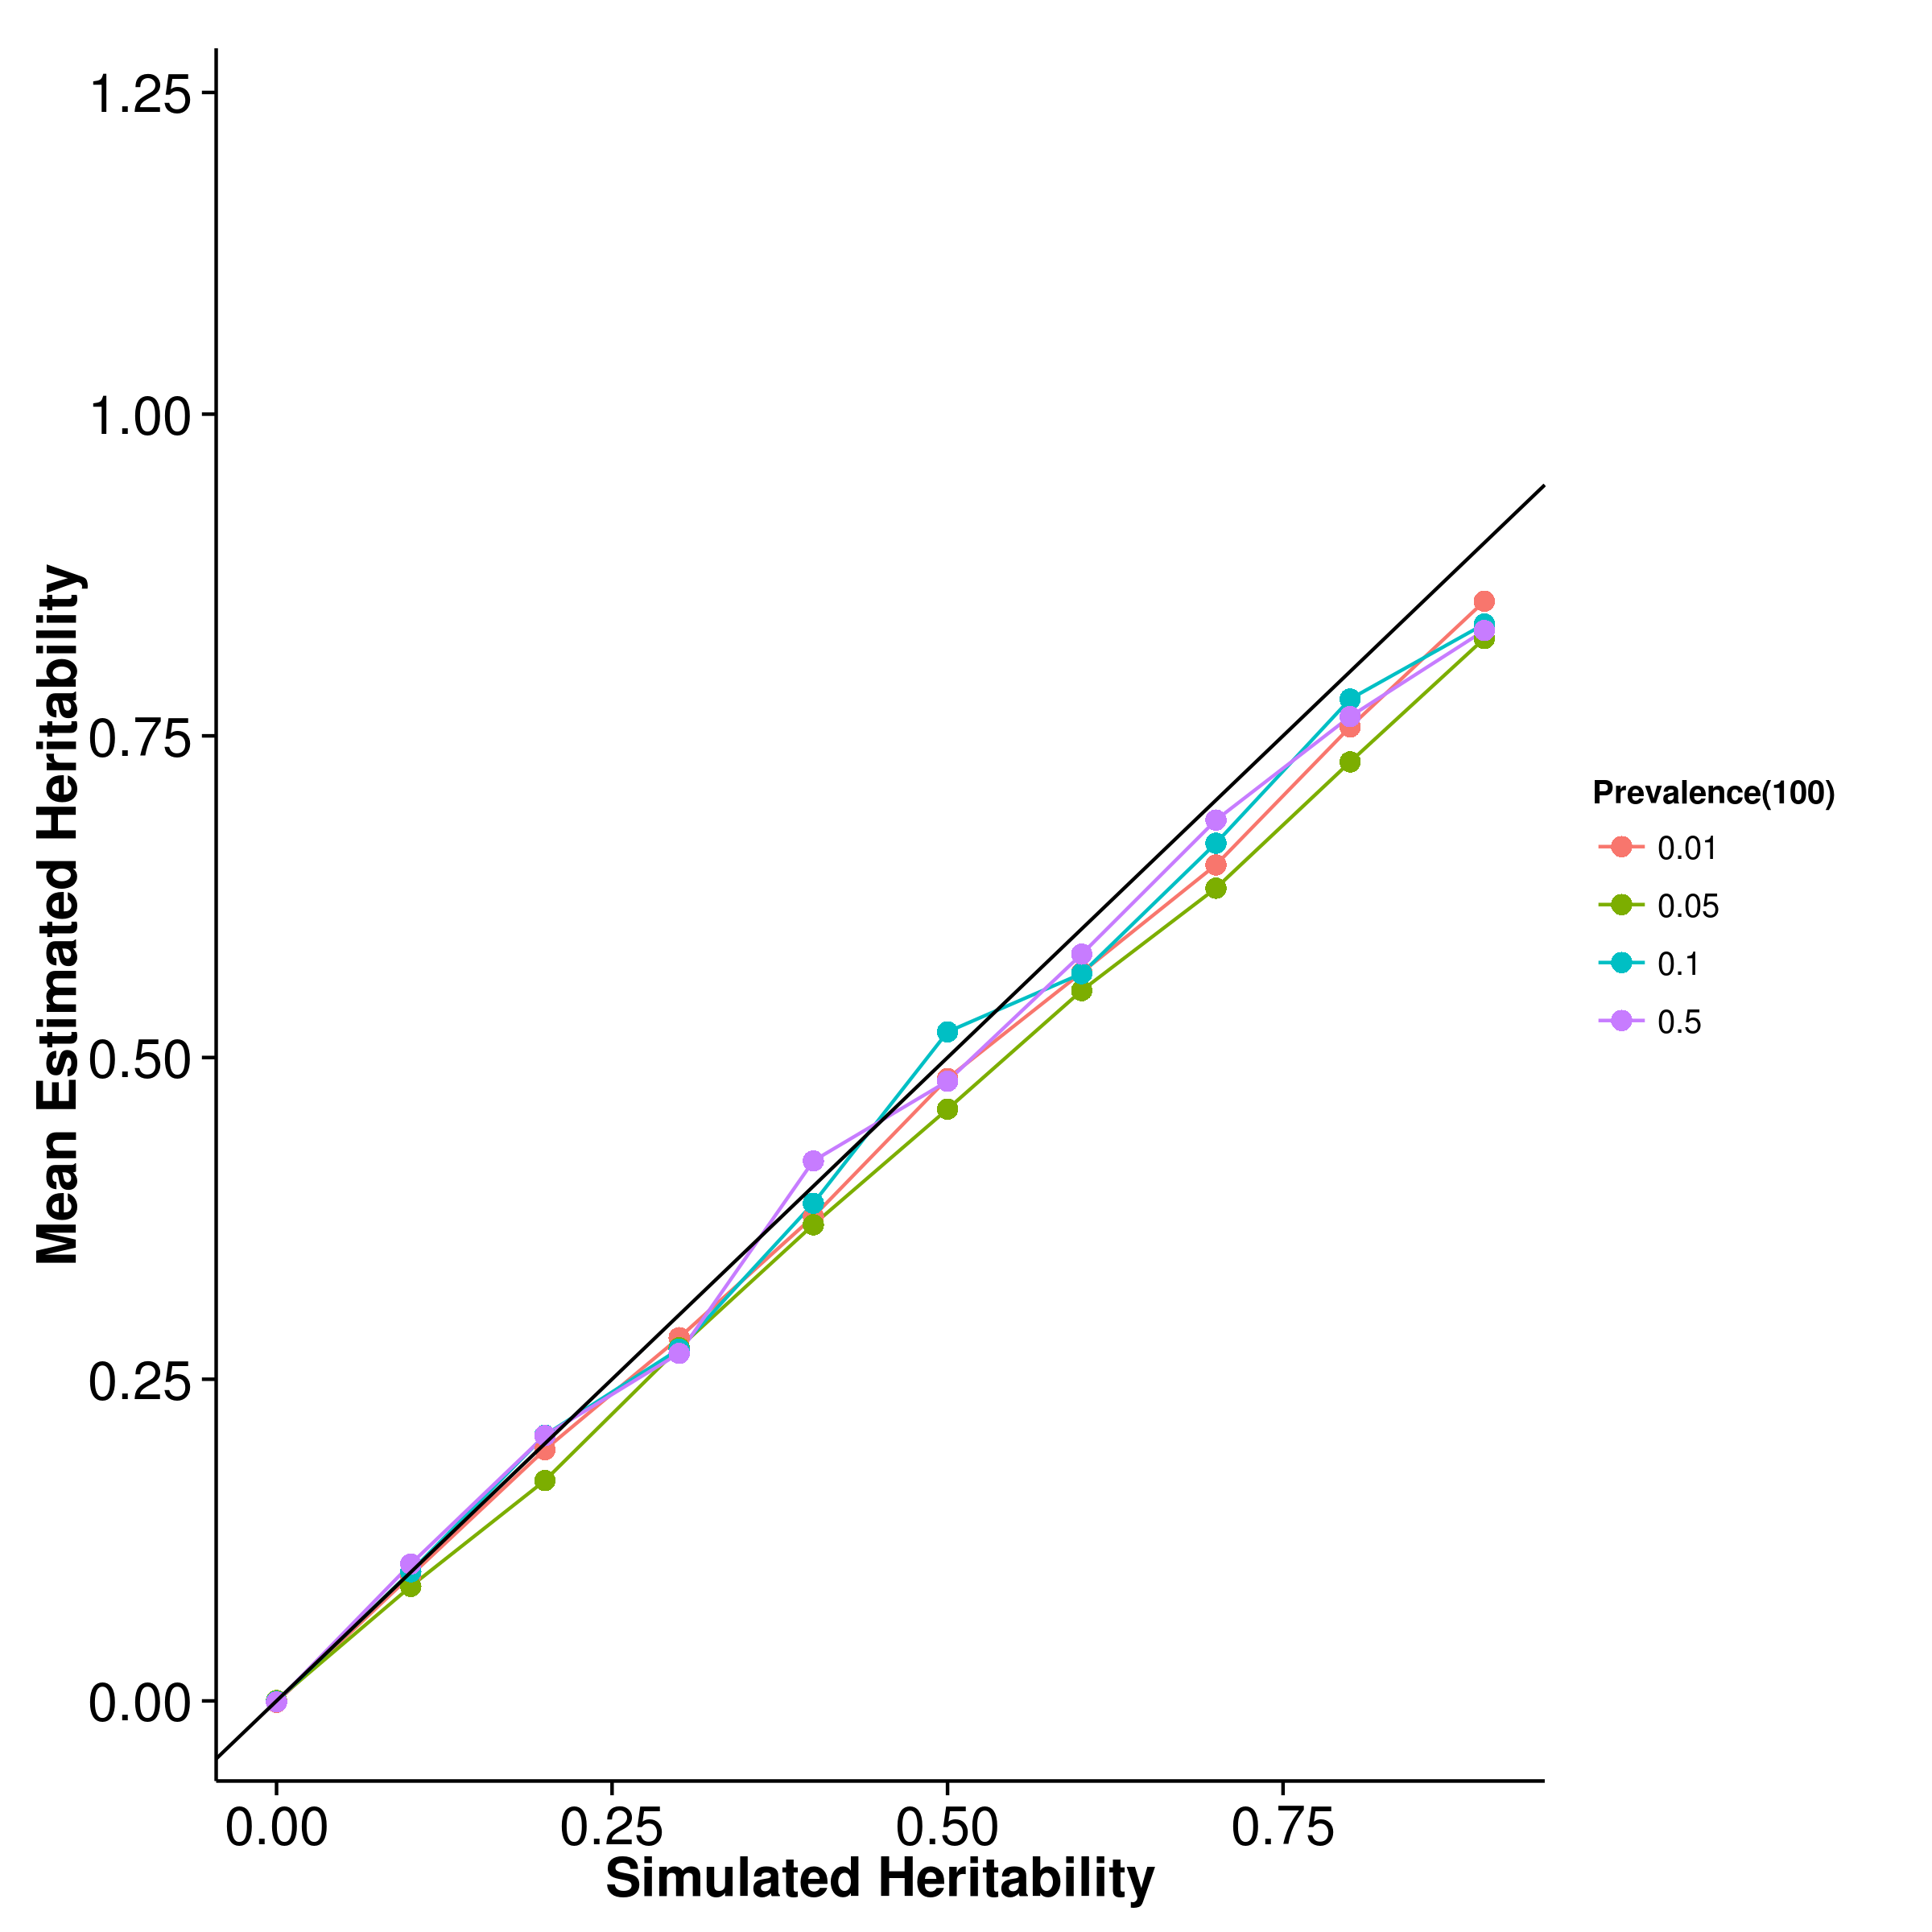
\includegraphics{figure/he_summary/cc_100c/ldscIn_CC_Random_mean.png}}
				\label{fig:ldscInCCRandMean}
			}
			\caption[Case Control with Random Effect Size Simulation Result(Mean)]
			{Mean of results from case control simulation with random effect size simulation.
				The performance of \gls{gcta} was as suggested by \citet{Golan2014} where there was an underestimation as prevalence decreases.
				On the other hand, \gls{ldsc} were upwardly biased when a fixed intercept was used and this bias was corrected when an estimation of intercept was allowed.
				\gls{shrek} does not seems to as sensitive to change in prevalence and the estimation were relatively robust.
				} 
			\label{fig:CCRandMean}
		\end{figure}
		
		\begin{figure}
			\centering
			\subfloat[SHREK]{
				\scalebox{.4}{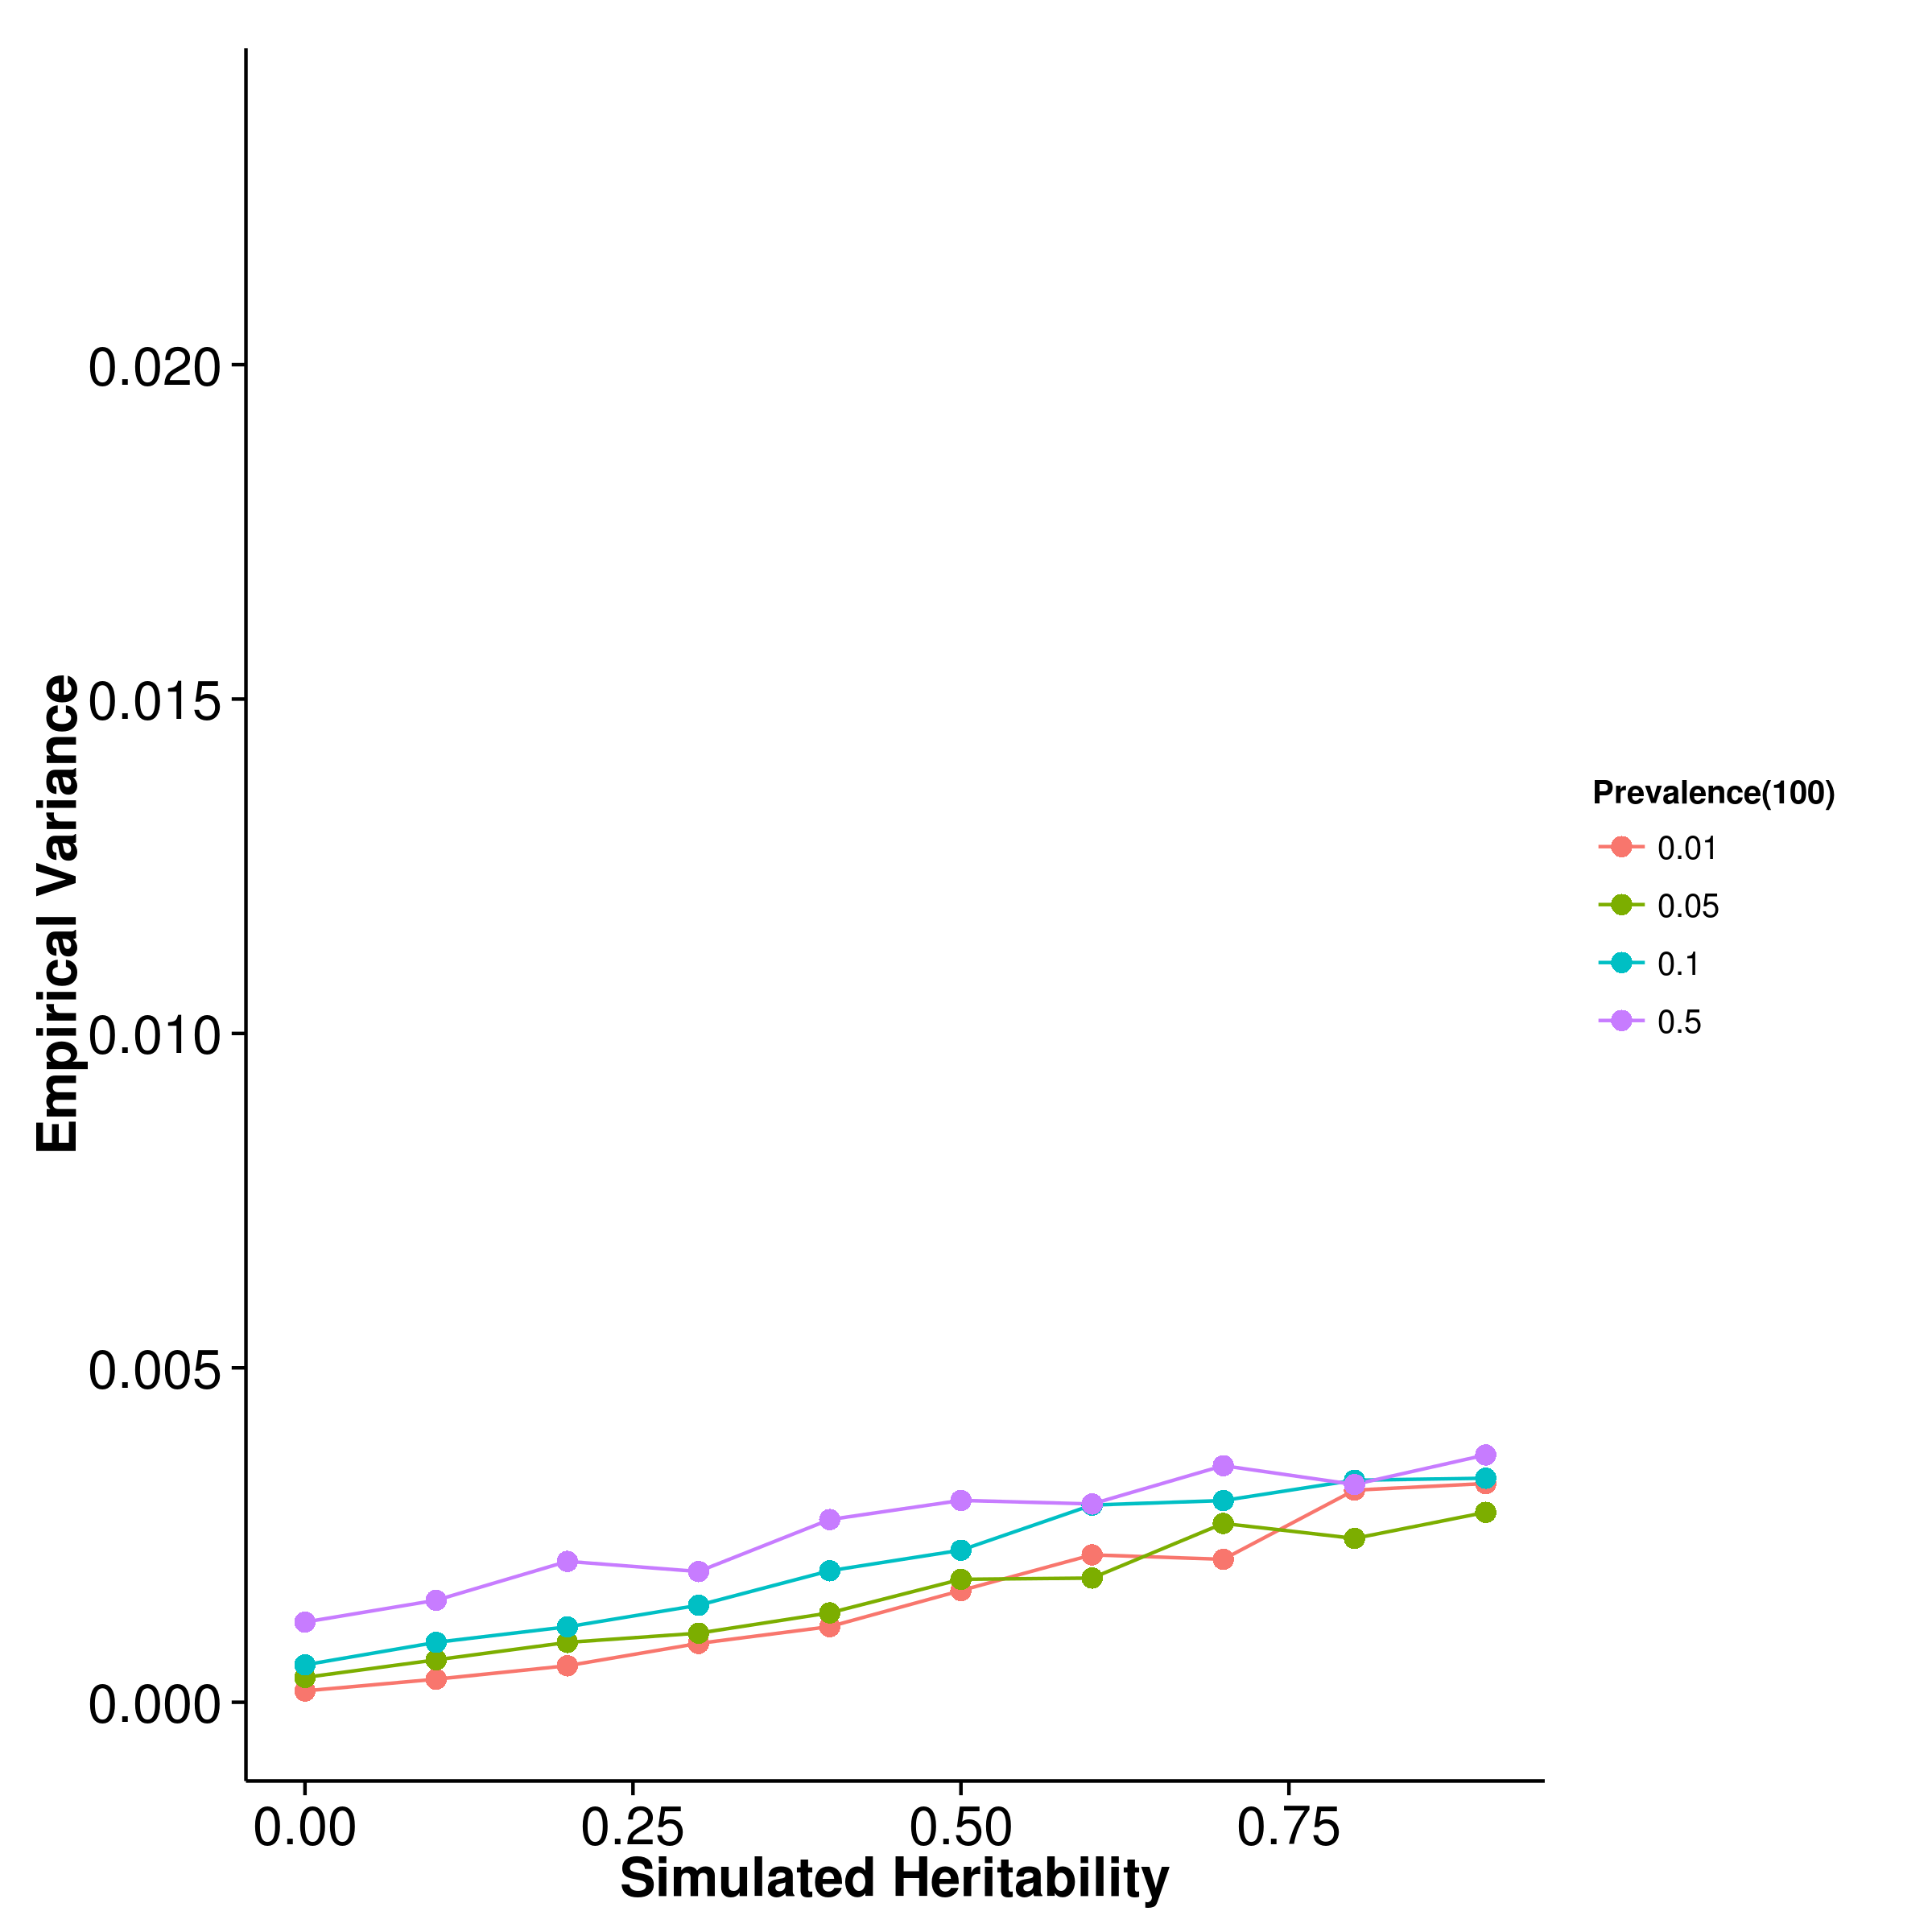
\includegraphics{figure/he_summary/cc_100c/shrek_CC_Random_sd.png}}
				\label{fig:shrekCCRandVar}
			}
			\subfloat[GCTA]{
				\scalebox{.4}{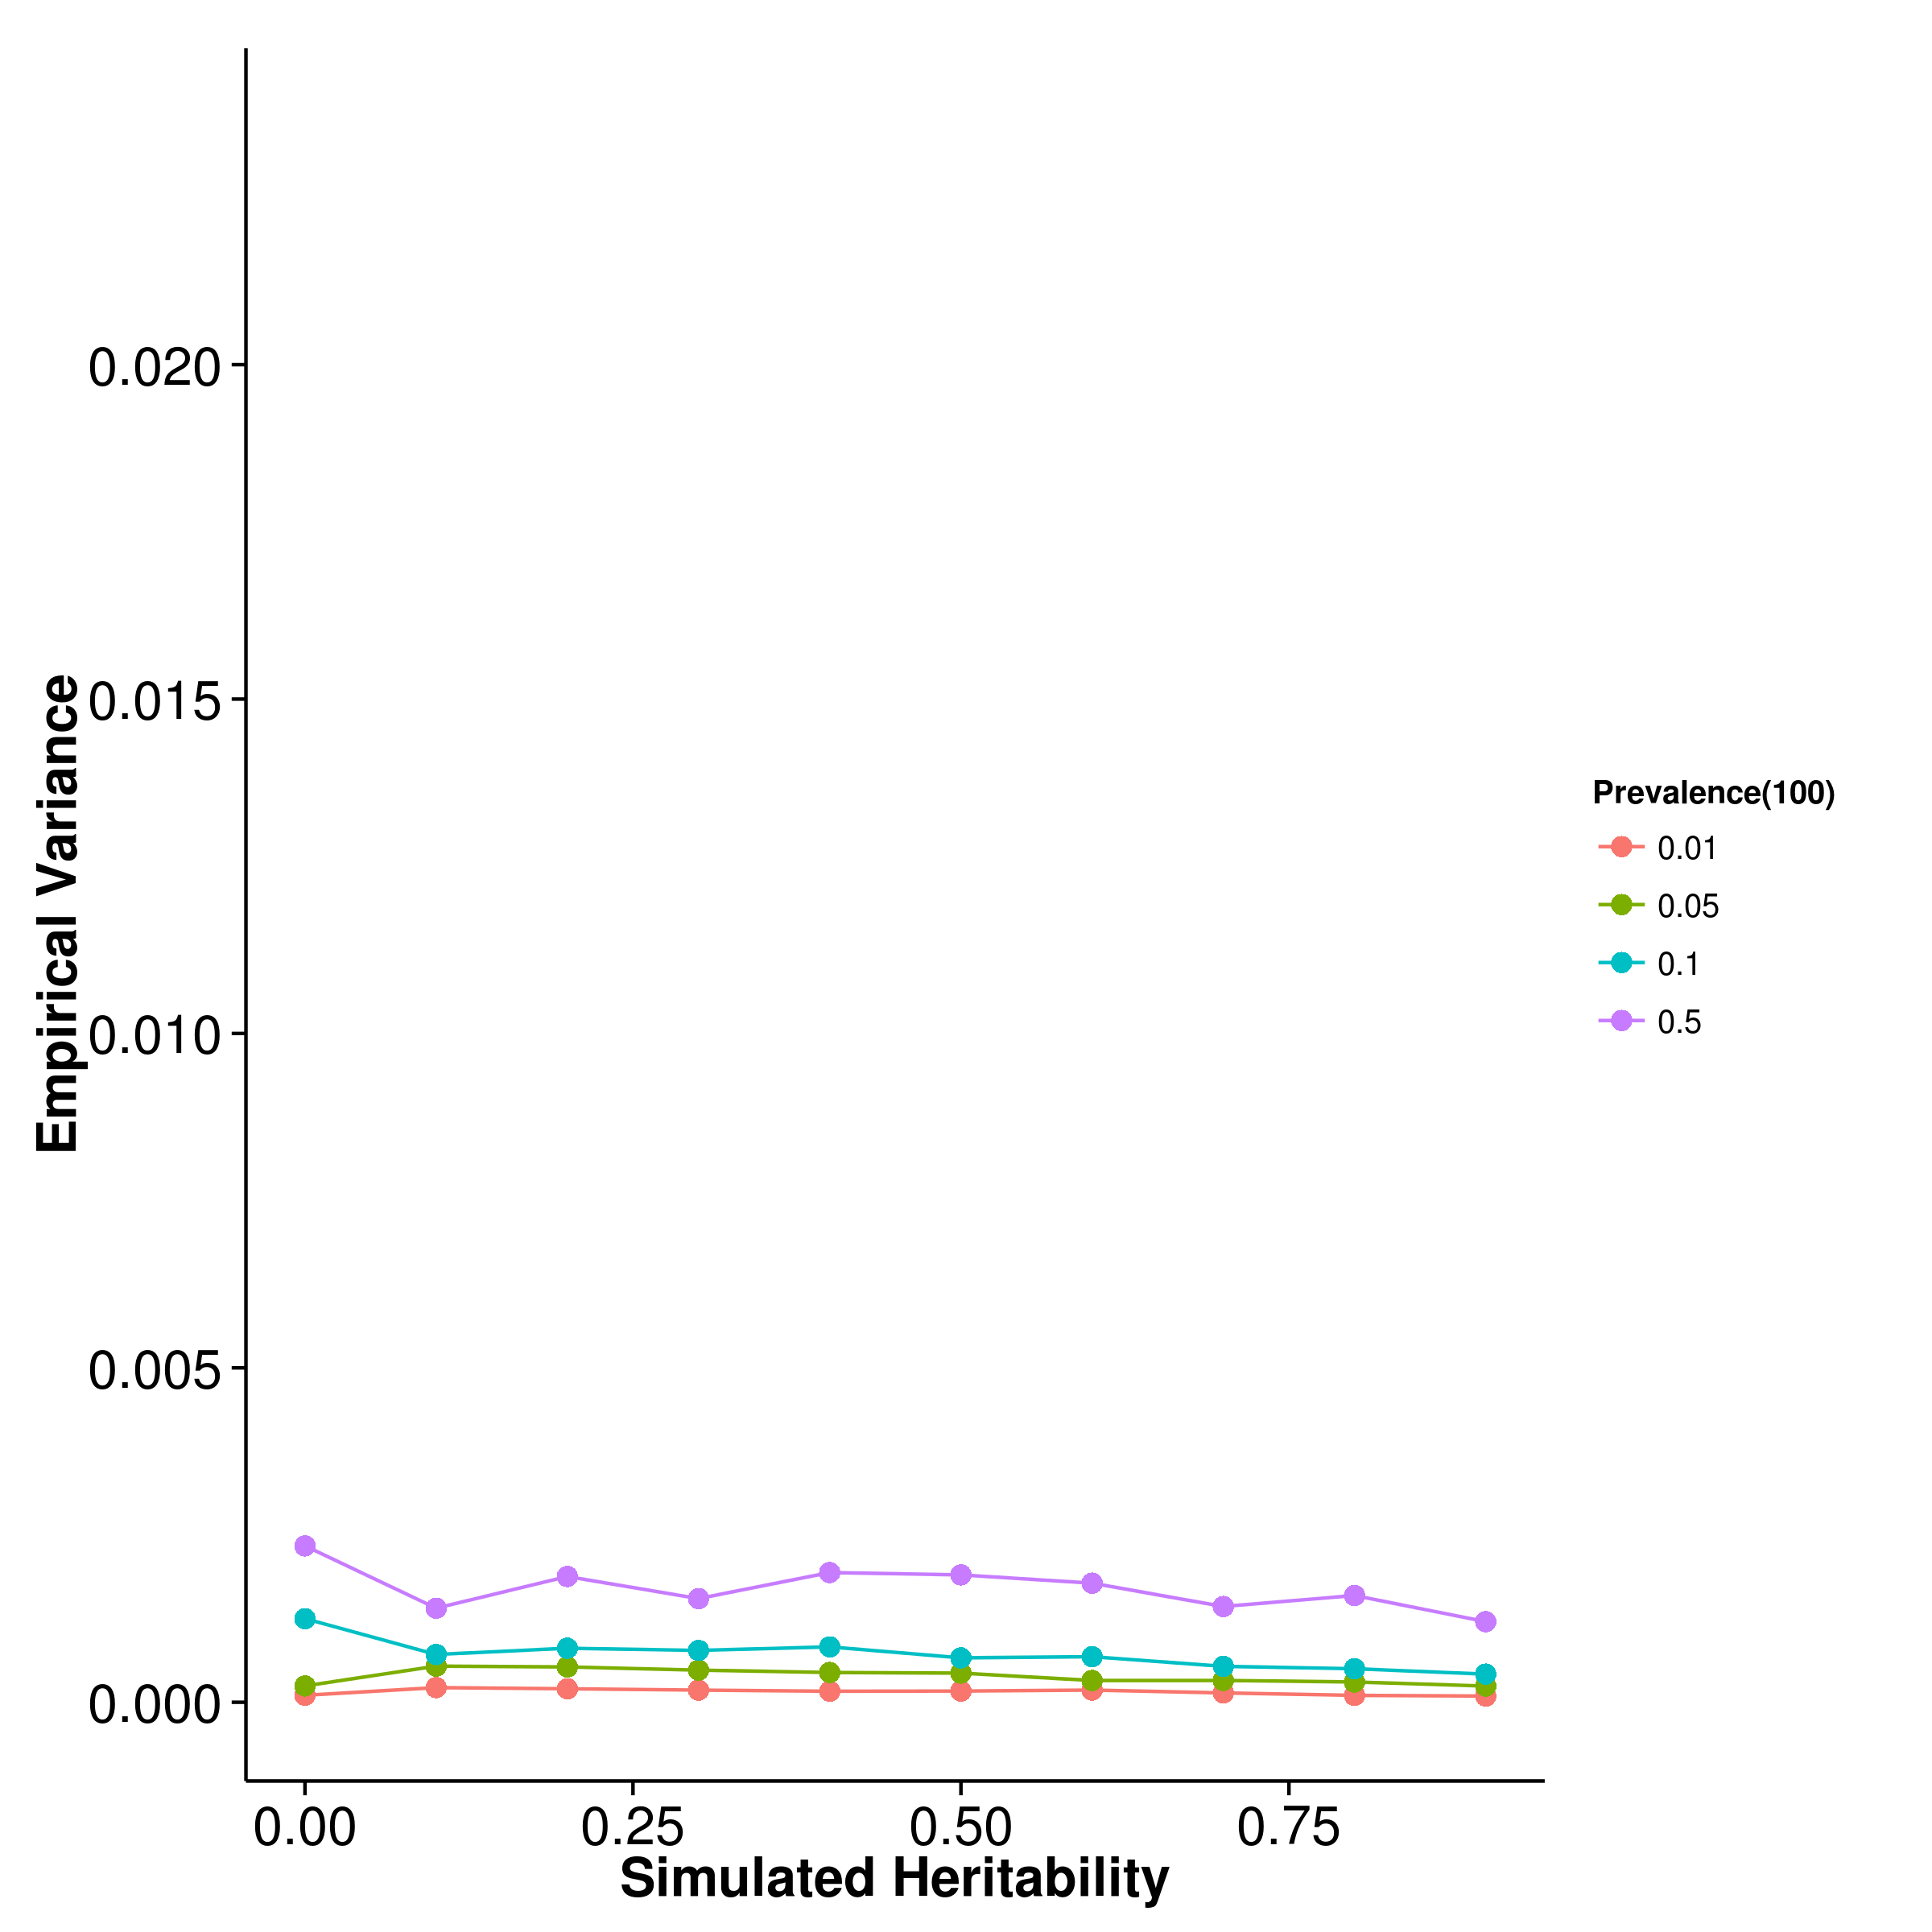
\includegraphics{figure/he_summary/cc_100c/gcta_CC_Random_sd.png}}
				\label{fig:gctaCCRandVar}
			}\\
			\subfloat[LDSC with fix intercept]{
				\scalebox{.4}{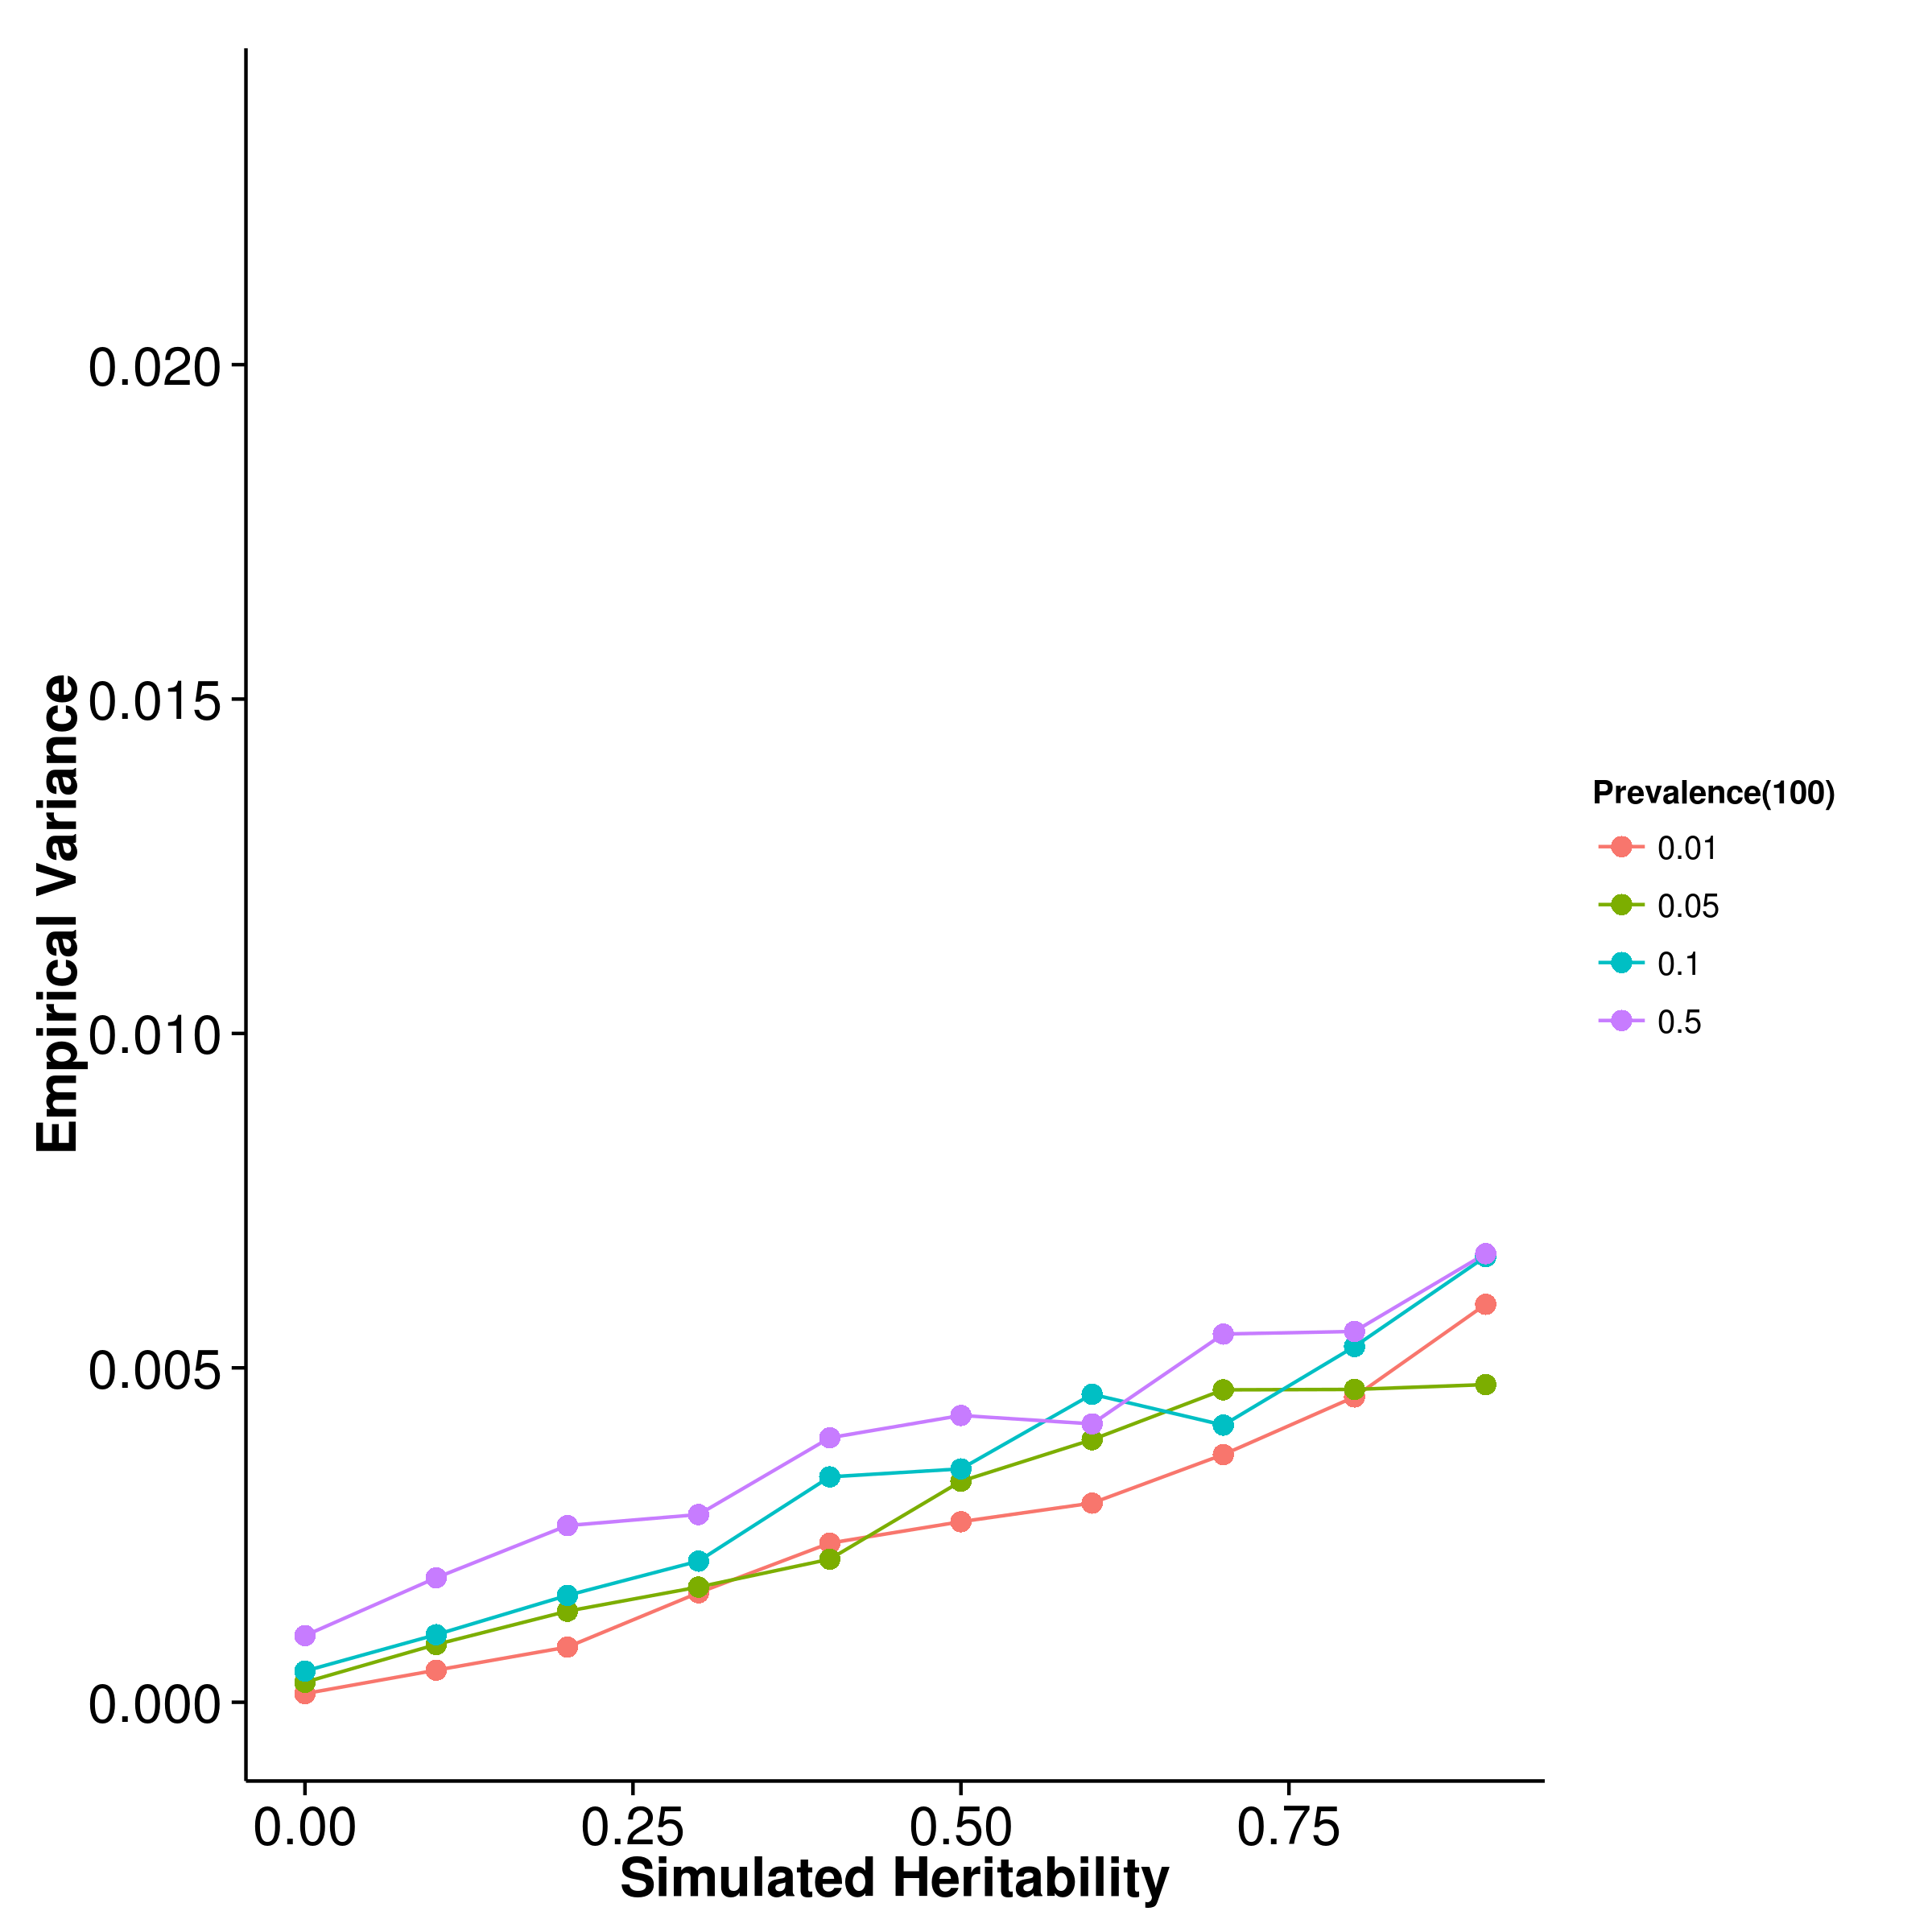
\includegraphics{figure/he_summary/cc_100c/ldsc_CC_Random_sd.png}}
				\label{fig:ldscCCRandVar}
			}
			\subfloat[LDSC with intercept estimation]{
				
				\scalebox{.4}{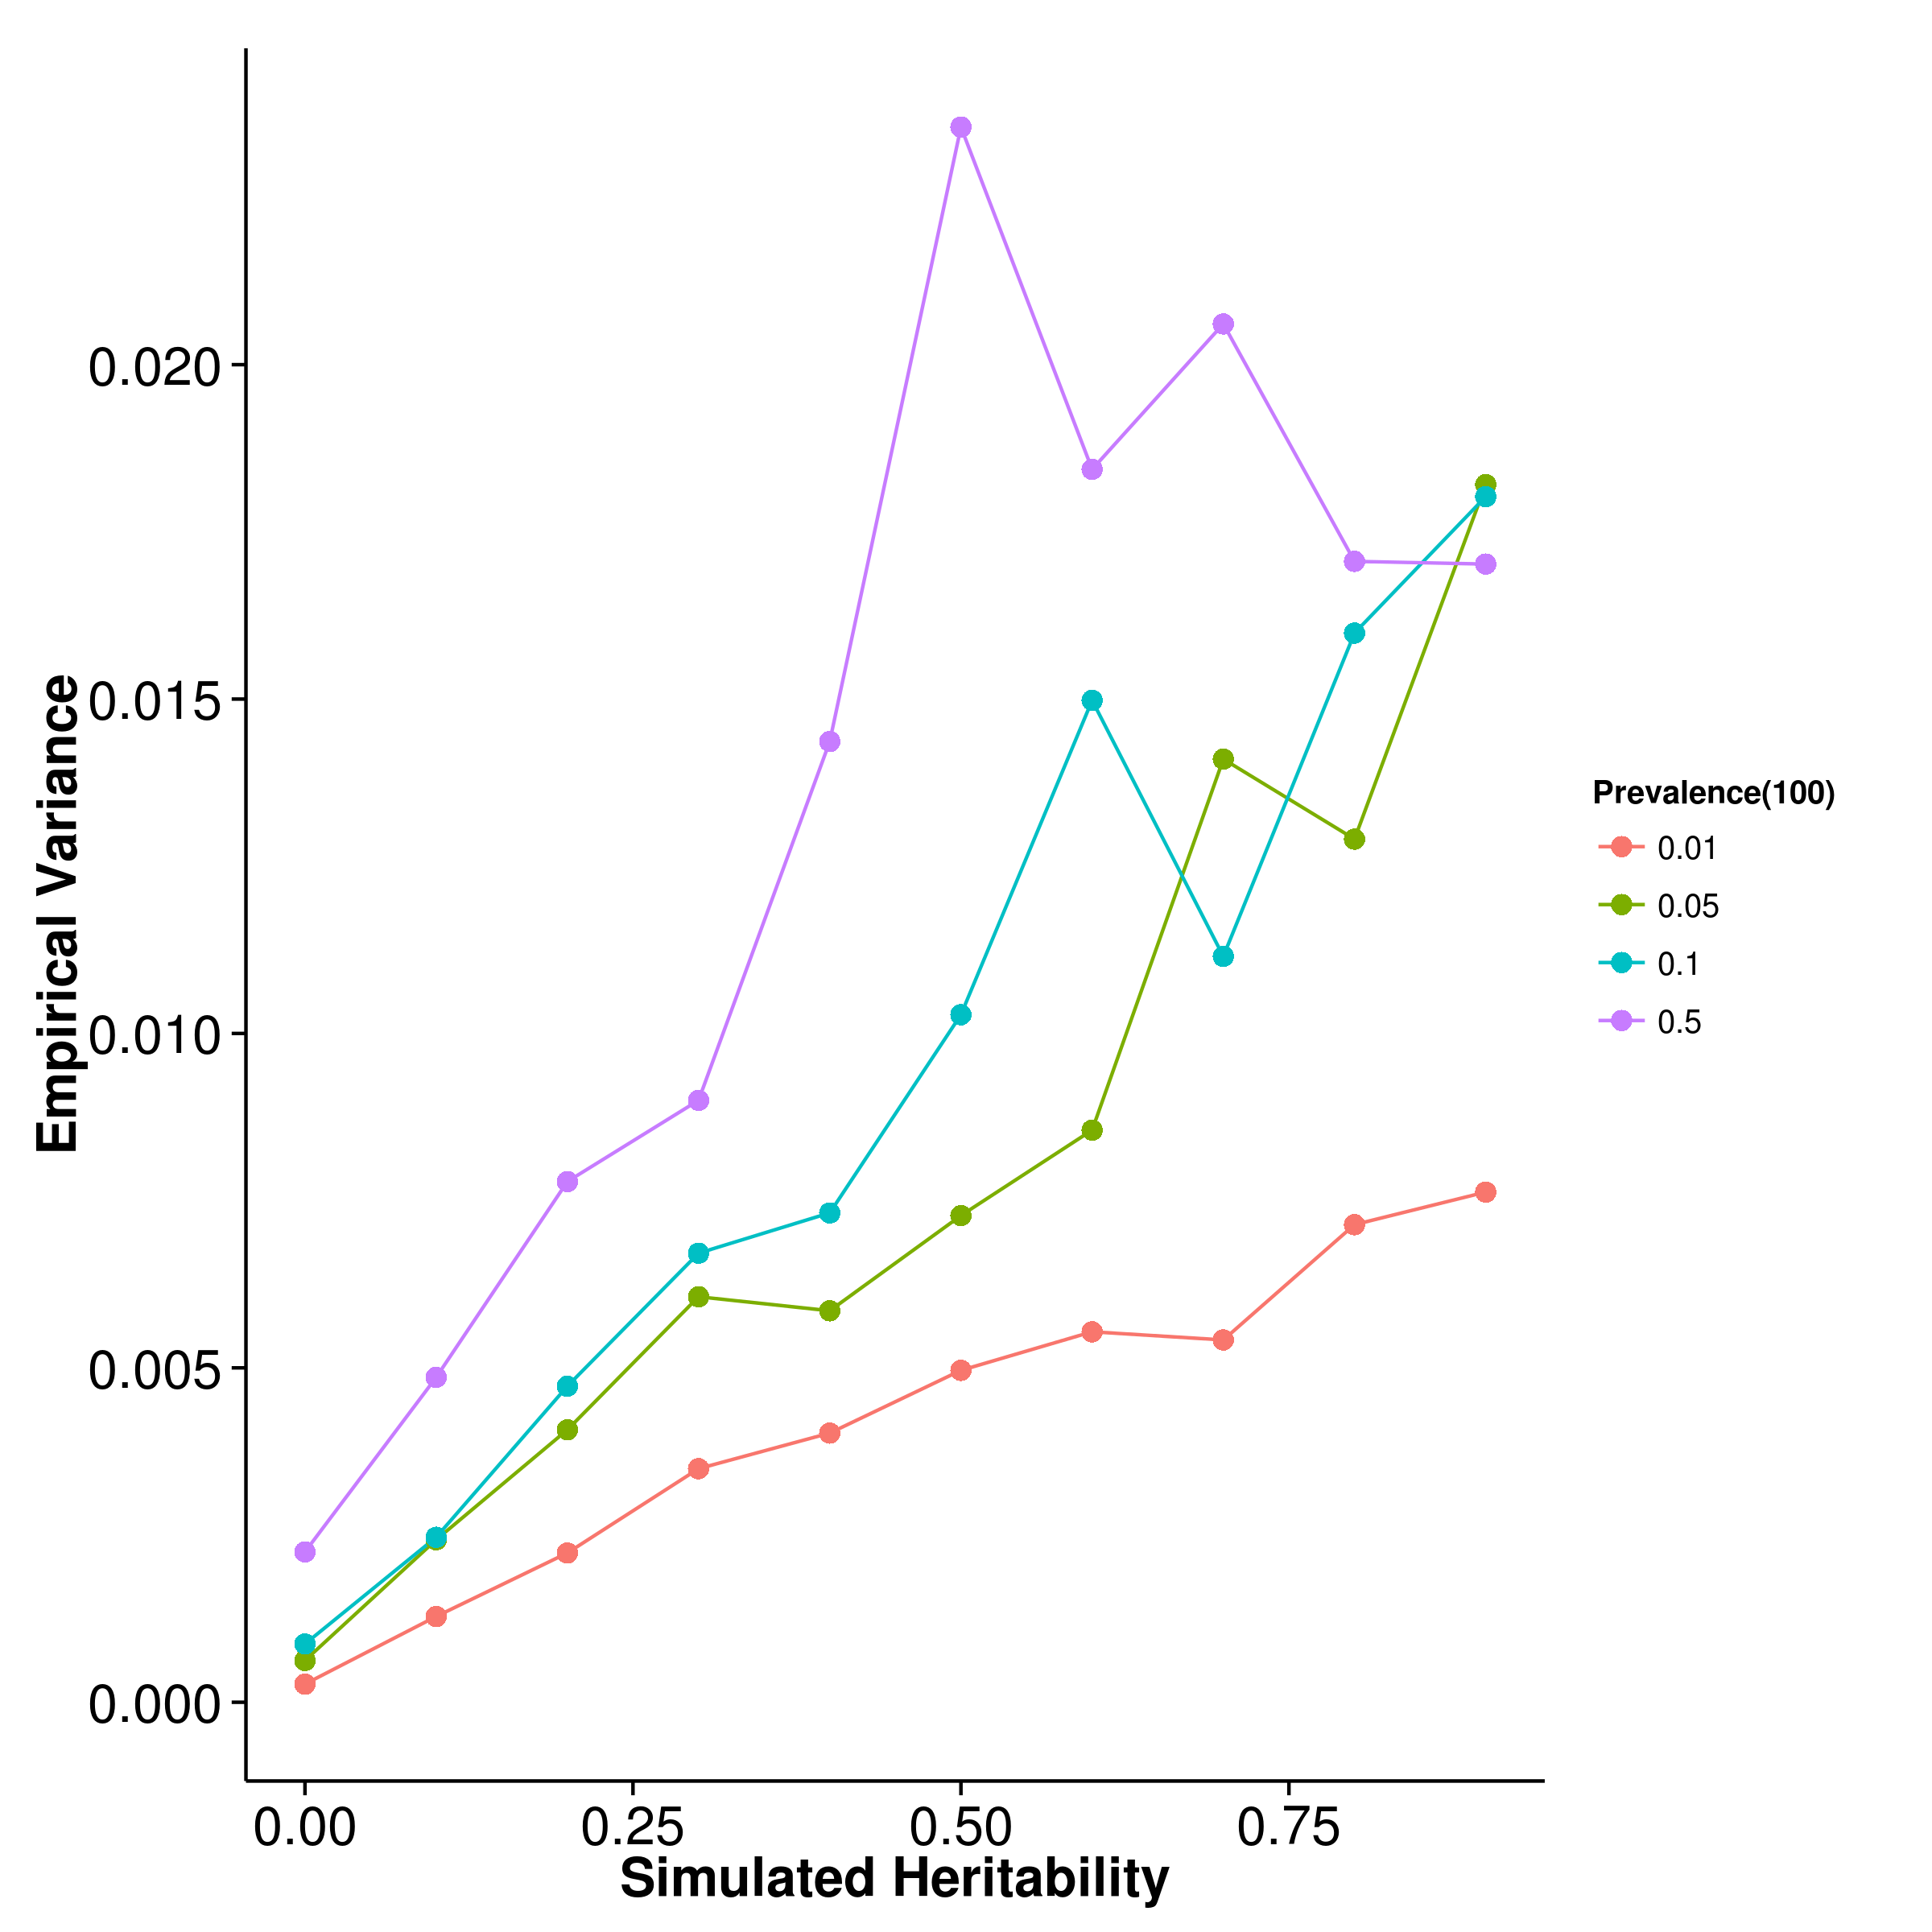
\includegraphics{figure/he_summary/cc_100c/ldscIn_CC_Random_sd.png}}
				\label{fig:ldscInCCRandVar}
			}
			\caption[Case Control with Random Effect Size Simulation Result(Variance)]
			{Variance of results from case control simulation with random effect size simulation.
				It was clear that the prevalence affects the variance of estimation where a larger variance tends to increase the variance of estimation.
				Again, \gls{gcta} has the lowest variance, however, unlike in the quantitative trait simulation, \gls{shrek} has a lower average variance when compared to \gls{ldsc} with fixed intercept.
				Nonetheless, it was important to remember that in case control simulation, a much smaller amount of \glspl{SNP} was used, thus the results was not directly comparable to results from the quantitative simulation.
			} 
			\label{fig:CCRandVar}
		\end{figure}
		
		
		\begin{figure}
			\centering
			\subfloat[SHREK]{
				\scalebox{.4}{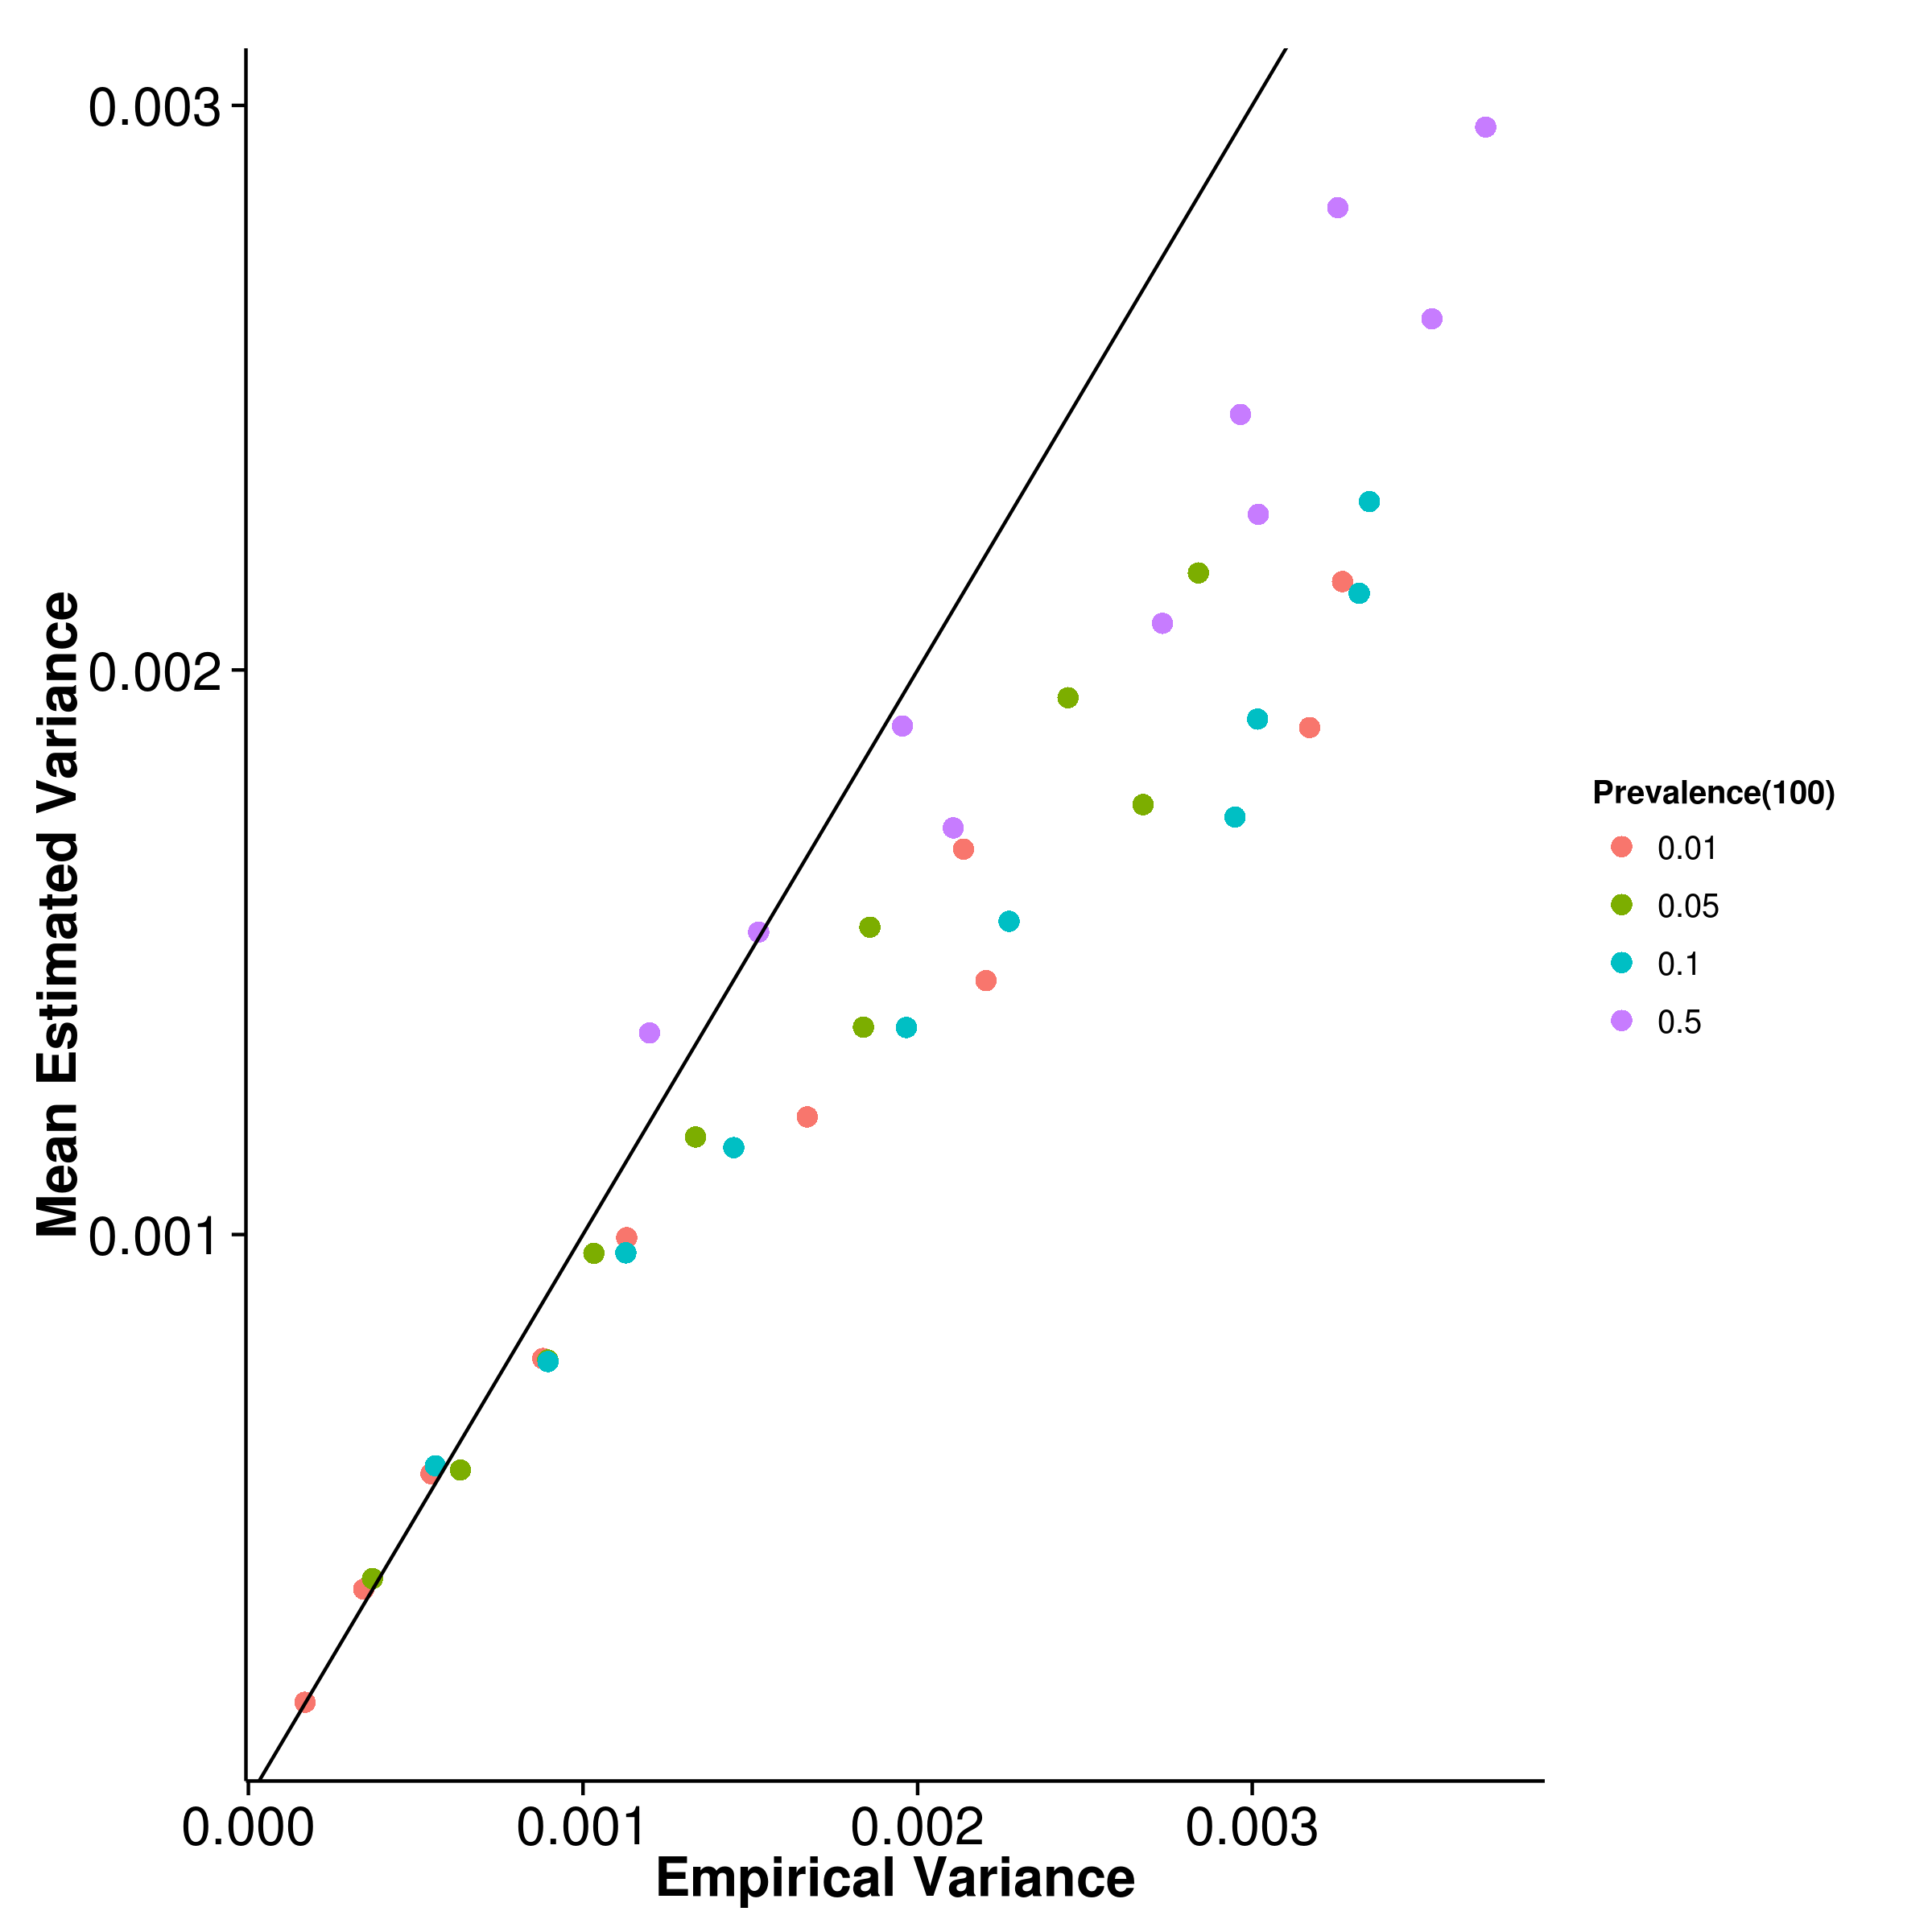
\includegraphics{figure/he_summary/cc_100c/shrek_CC_Random_sdCom.png}}
				\label{fig:shrekCCRandVarCom}
			}
			\subfloat[GCTA]{
				\scalebox{.4}{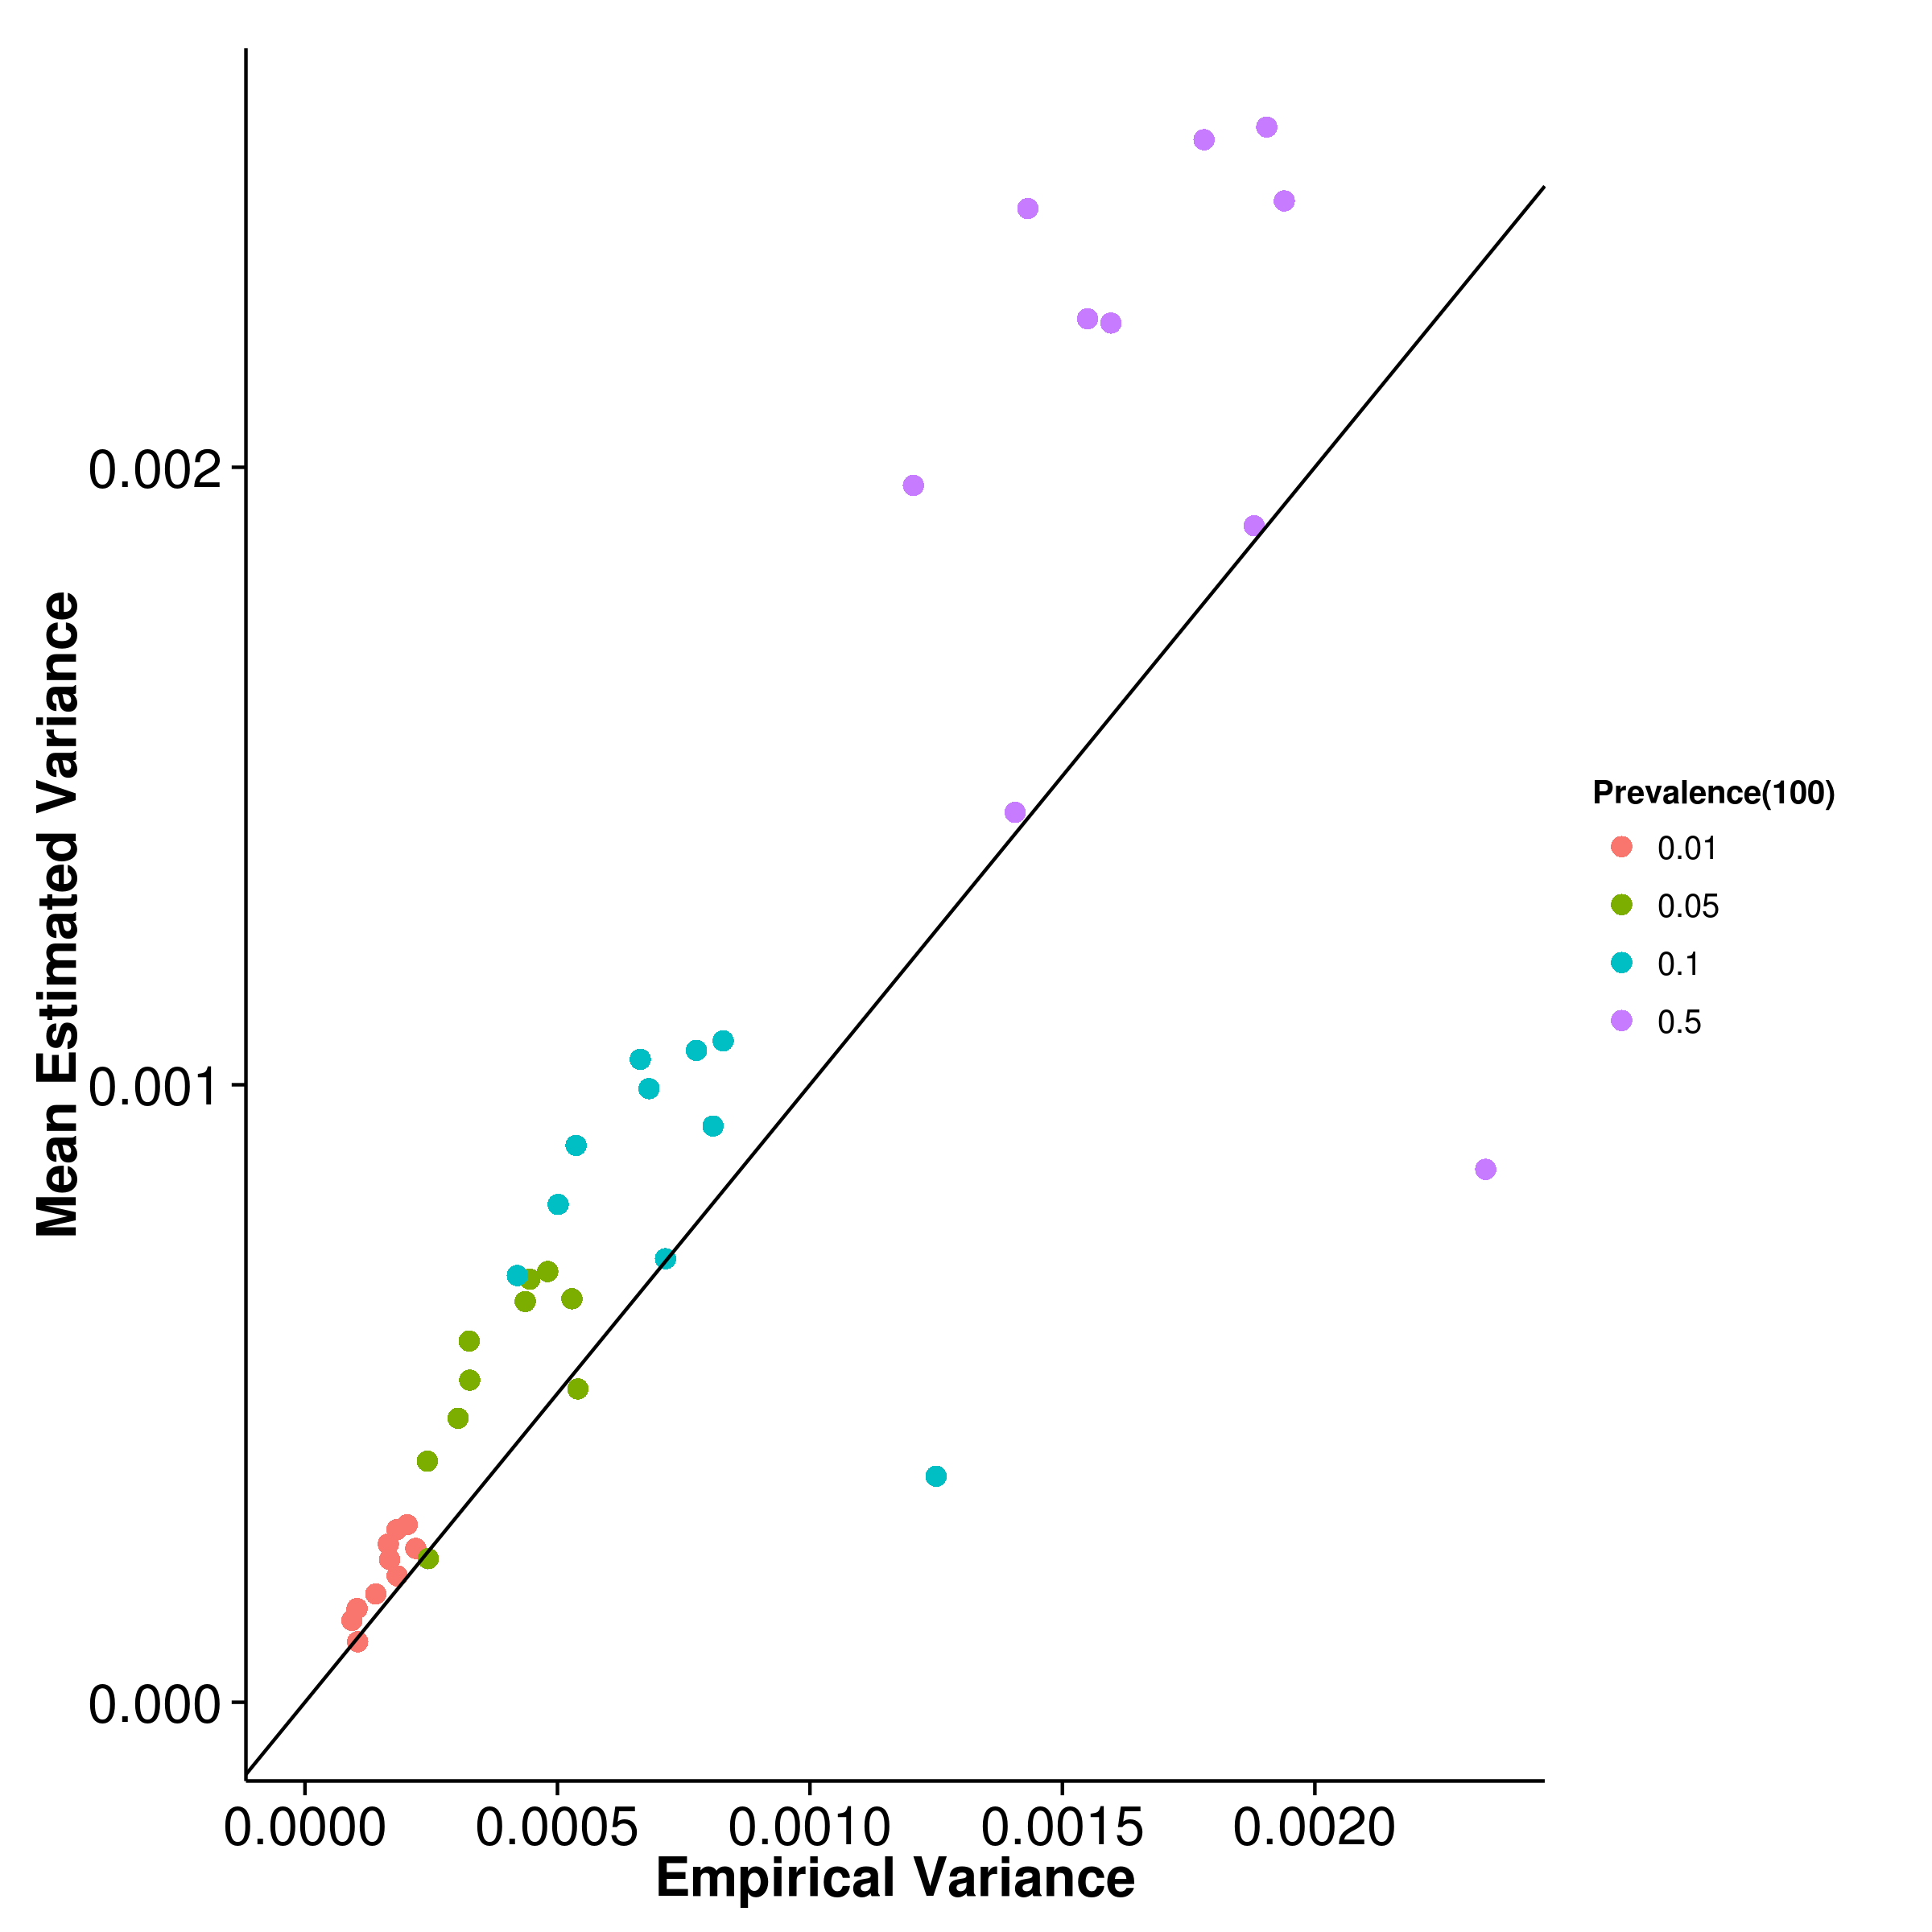
\includegraphics{figure/he_summary/cc_100c/gcta_CC_Random_sdCom.png}}
				\label{fig:gctaCCRandVarCom}
			}\\
			\subfloat[LDSC with fix intercept]{
				\scalebox{.4}{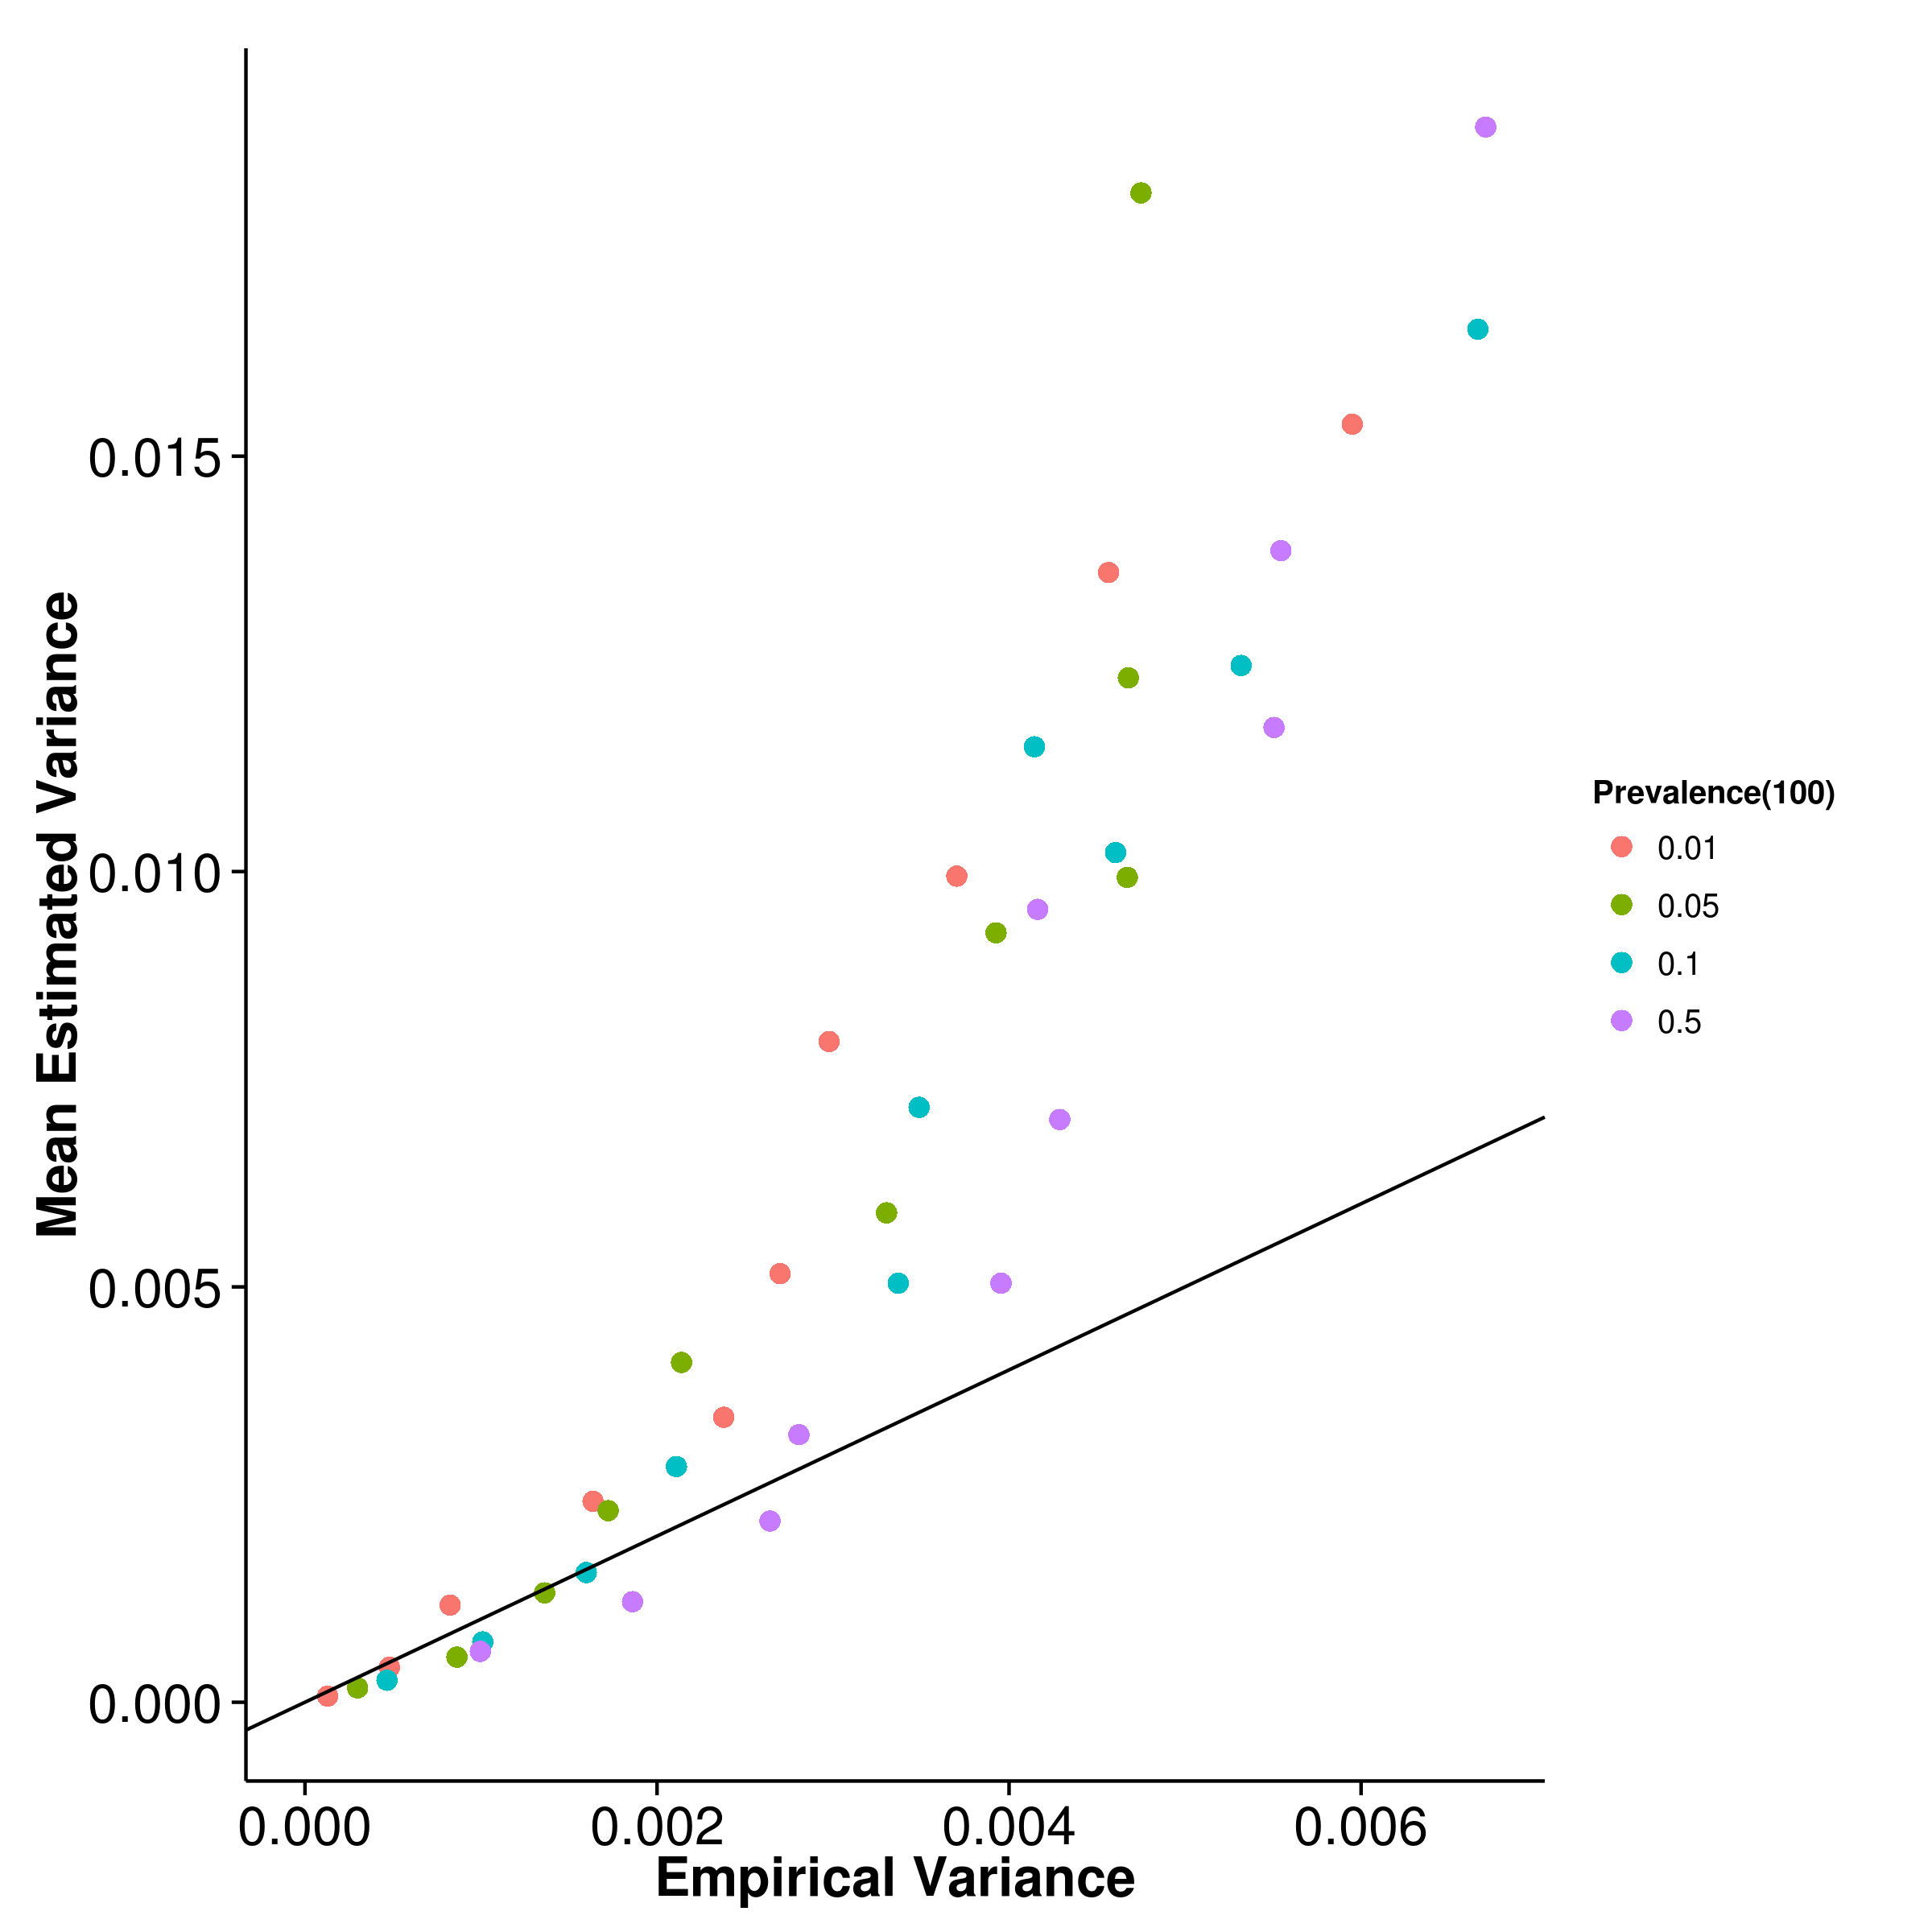
\includegraphics{figure/he_summary/cc_100c/ldsc_CC_Random_sdCom.png}}
				\label{fig:ldscCCRandVarCom}
			}
			\subfloat[LDSC with intercept estimation]{
				
				\scalebox{.4}{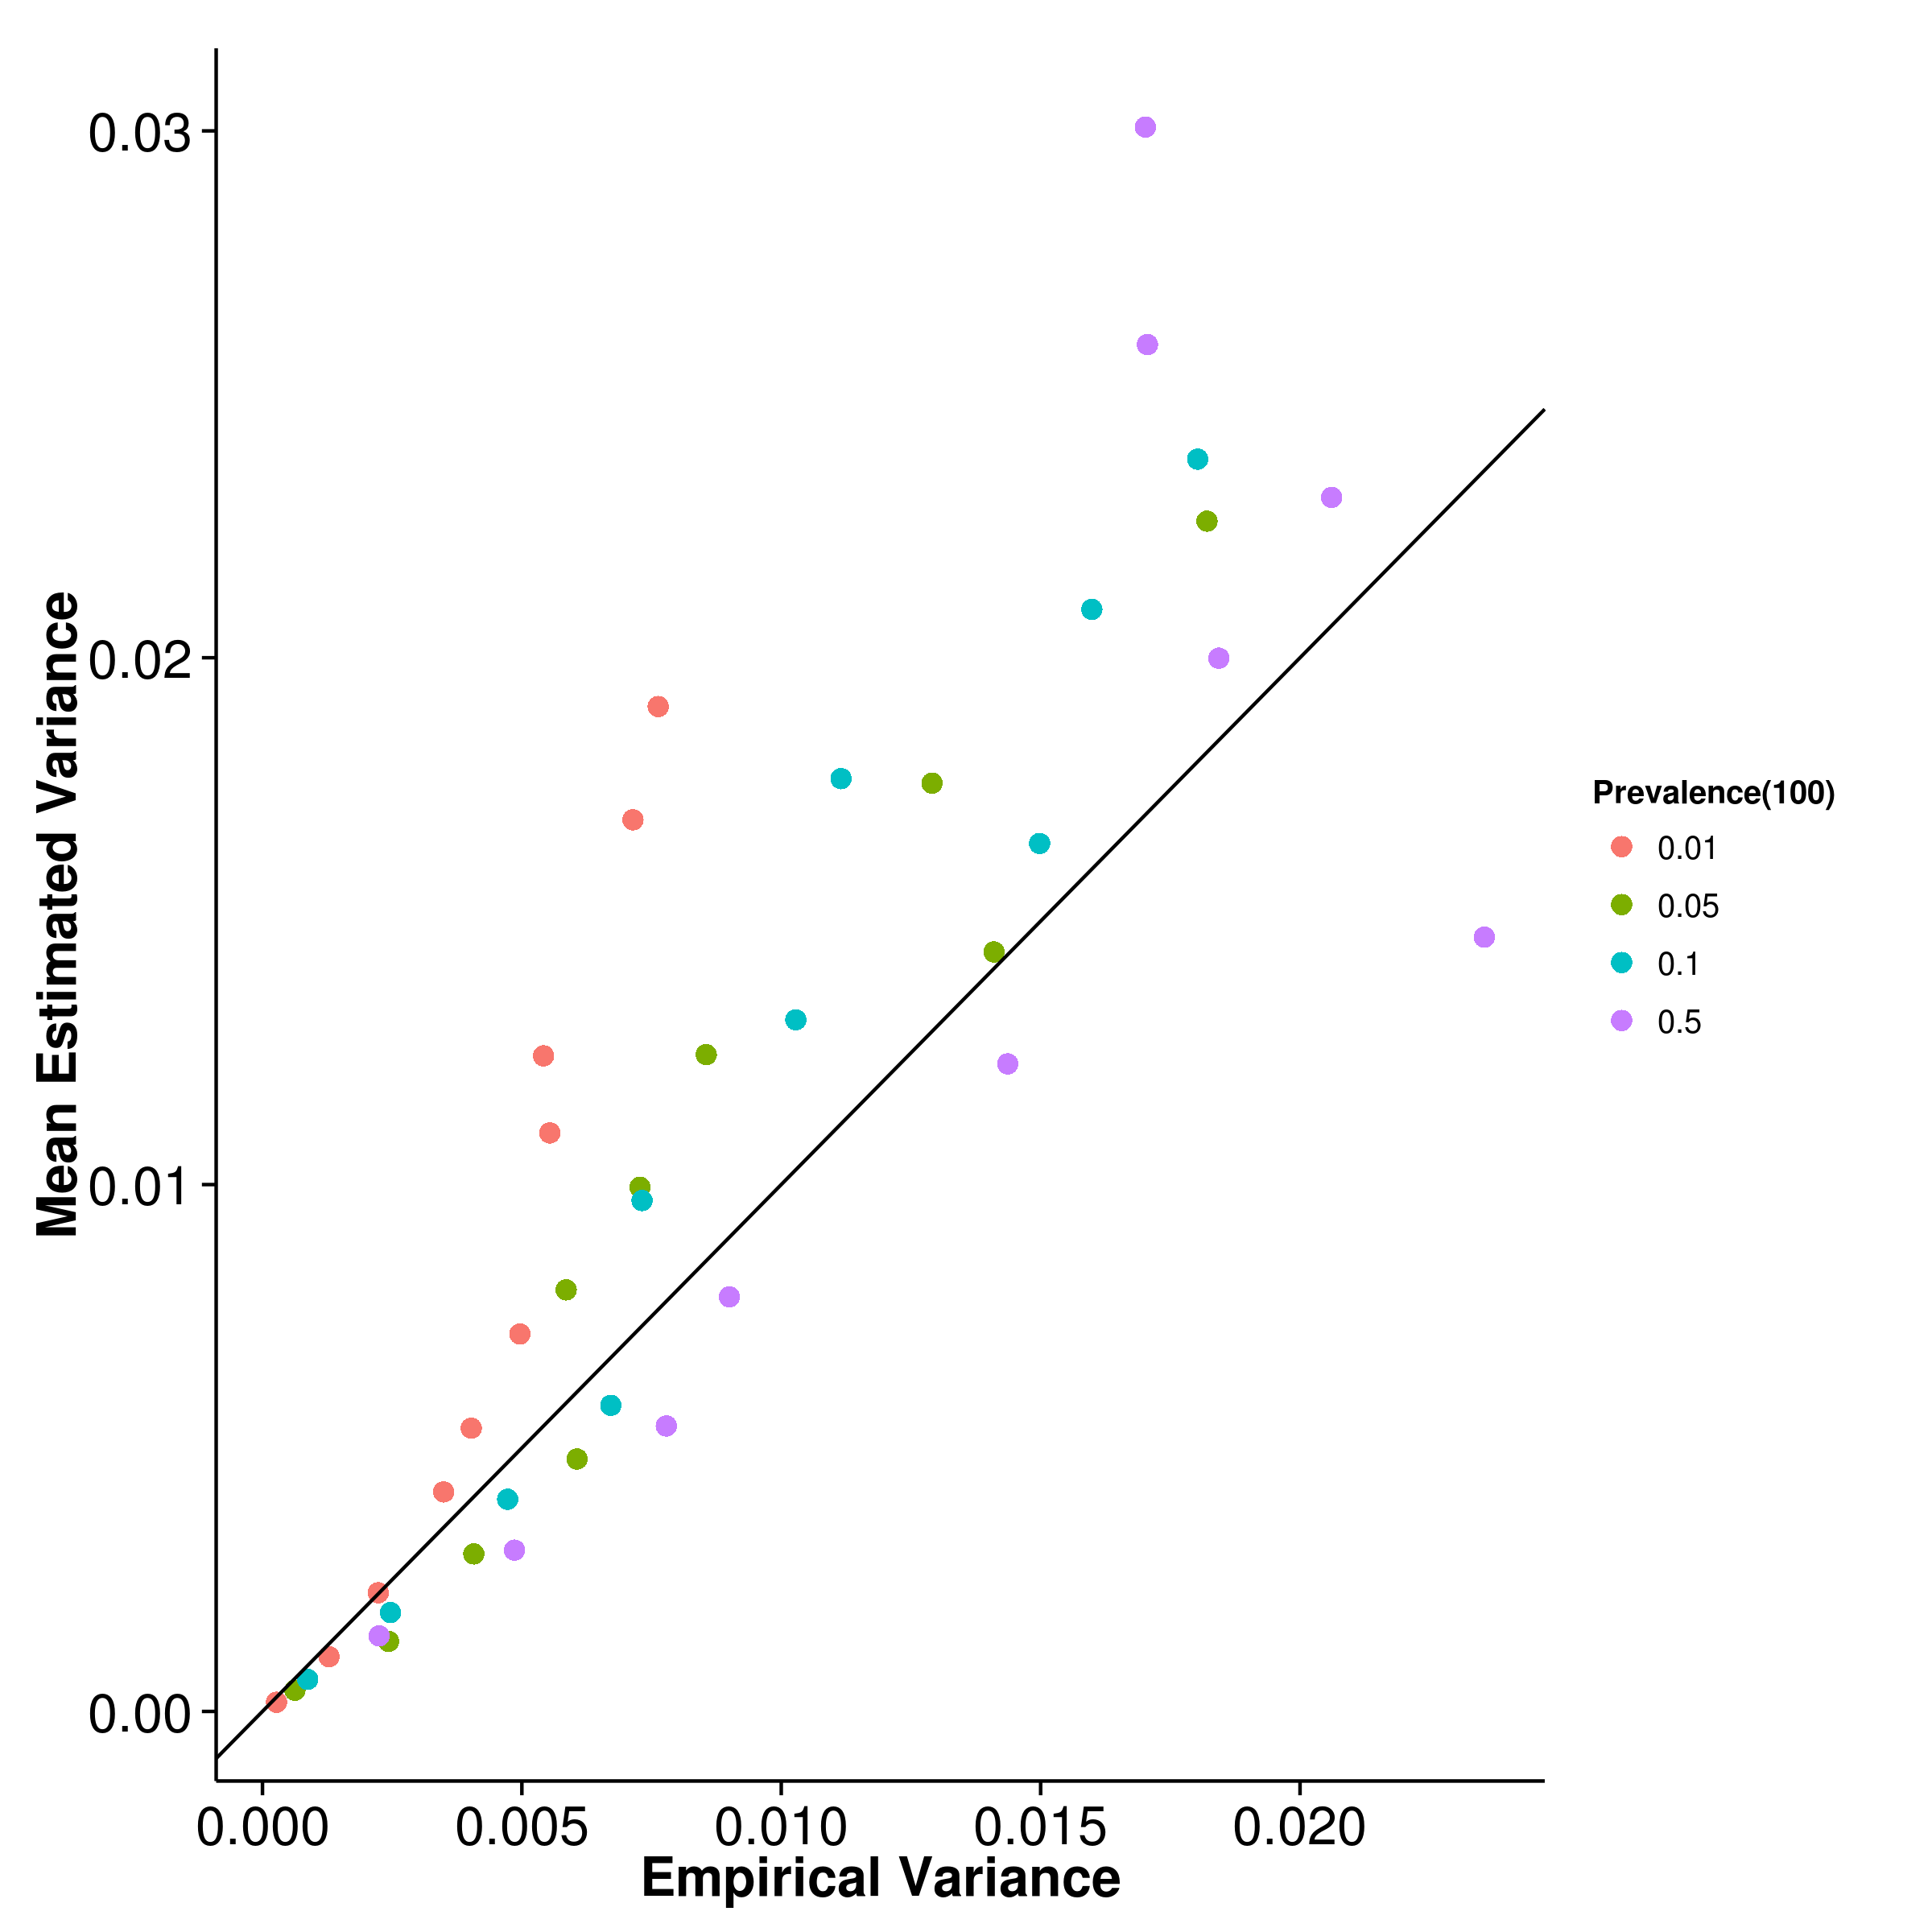
\includegraphics{figure/he_summary/cc_100c/ldscIn_CC_Random_sdCom.png}}
				\label{fig:ldscInCCRandVarCom}
			}
			\caption[Case Control with Random Effect Size Simulation Result(Estimated Variance)]
			{Estimated variance of results from case control simulation with random effect size simulation when compared to empirical variance.
				From the quantitative trait simulation with random effect size(\cref{fig:QtRandVarCom}), it was observed that the variance estimation of \gls{shrek} and \gls{gcta} were rater accurate.
				Similarly, in the case control simulation with 100 causal \glspl{SNP}, it was observed that the variance estimation of \gls{shrek} and \gls{gcta} were close to the empirical variance with slight bias.
				A large up-ward bias was observed for \gls{ldsc} with fixed intercept estimation but the bias was less when \gls{ldsc} was allowed to estimate the intercept.s
			} 
			\label{fig:CCRandVarCom}
		\end{figure}